\documentclass[usenames, dvipsnames, aspectratio=169]{beamer}

%%%%%
%%%%%
%%%%%
%%%%%
%%%%%

\usepackage{xcolor}
\usepackage{tikz}
\usetikzlibrary{backgrounds}
\usetikzlibrary{arrows, shapes}
\usetikzlibrary{tikzmark}
\usetikzlibrary{calc}
\usetikzlibrary{positioning}
\usetikzlibrary{shadows}
\usetikzlibrary{trees, mindmap}
\usetikzlibrary{lindenmayersystems}

\usepackage{pgfplots}
\pgfplotsset{compat=newest}

\usepackage{tcolorbox}

\newcommand{\highlight}[2]{\colorbox{#1!17}{$\displaystyle #2$}}
\newcommand{\highlightdark}[2]{\colorbox{#1!47}{$\displaystyle #2$}}
\renewcommand{\highlight}[2]{\colorbox{#1!17}{#2}}
\renewcommand{\highlightdark}[2]{\colorbox{#1!47}{#2}}

\usepackage[utf8]{inputenc}
\usepackage[english]{babel}

\usepackage{amsmath, amssymb, amsfonts}

\usepackage[]{bm}
\usepackage[]{nicefrac}

\usepackage{graphicx}
\usepackage{multimedia}

\usepackage{xspace}

\newcommand{\lap}{\nabla^2}

%%%%%
%%%%%
%%%%%
%%%%%
%%%%%





\usetheme{default}
\usefonttheme{professionalfonts}
\setbeamertemplate{navigation symbols}{}
\setbeamertemplate{itemize items}[circle]
\setbeamercolor{itemize item}{fg=white}

\setbeamerfont{title}{series=\bfseries, size=\normalfont\Large}
\setbeamercolor{title}{fg=white}

\setbeamerfont{author}{size=\normalfont\small}
\setbeamercolor{author}{fg=white}

\setbeamerfont{frametitle}{series=\bfseries, size=\normalfont}
\setbeamercolor{frametitle}{fg=white}

\setbeamerfont{framesubtitle}{size=\normalfont\large}
\setbeamercolor{framesubtitle}{fg=white}

\setbeamercolor{background canvas}{bg=black}
\setbeamercolor{normal text}{fg=white}

\setbeamercolor{local structure}{fg=white}





\graphicspath{{imgs/}}




%%%%%
%%%%%
%%%%%
%%%%%
%%%%%

\pgfdeclarelindenmayersystem{Koch curve}{
  \symbol{X}{\pgflsystemdrawforward}
  \rule{X -> X + X -- X + X}
}

\pgfdeclarelindenmayersystem{Three Half curve}{
  \symbol{X}{\pgflsystemdrawforward}
  \rule{X -> X + X - X - XX + X + X - X}
}

\pgfdeclarelindenmayersystem{Sierpinsky}{
  \symbol{X}{\pgflsystemdrawforward}
  \symbol{Y}{\pgflsystemdrawforward}
  \rule{X -> Y - X - Y}
  \rule{ Y -> X + Y + X}
}

\pgfdeclarelindenmayersystem{Hilbert curve}{
  \rule{L -> +RF-LFL-FR+}
  \rule{R -> -LF+RFR+FL-}
}


\title{A glimpse of fractal geometry}
\author{Jean-Christophe LOISEAU}
\institute{Arts \& Métiers Institute of Technology, January 2022}
\date{}

\begin{document}

\frame{\titlepage}

{
  \setbeamercolor{background canvas}{bg=white}
  \setbeamercolor{background canvas}{bg=white}
  \setbeamercolor{normal text}{fg=black}

  \usebeamercolor[fg]{normal text}

  \setbeamercolor{frametitle}{fg=black}
  \setbeamercolor{framesubtitle}{fg=black}
  \setbeamercolor{itemize item}{fg=black}

  \begin{frame}
    \vfill
    \centering
%    \large

    \begin{minipage}{.22\textwidth}
      \centering
      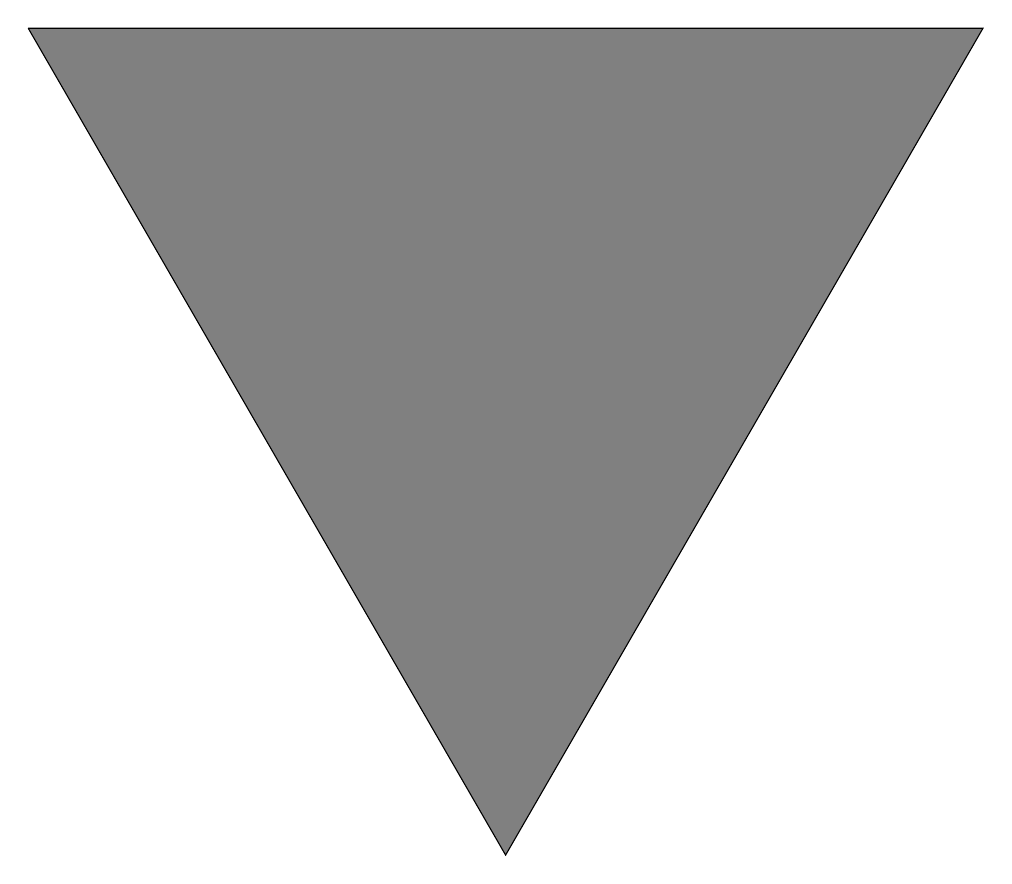
\begin{tikzpicture}
        \draw[thin, fill=gray] (0, 0) l-system[l-system={Koch curve, axiom=X--X--X, step=\textwidth, order=0, angle=60}];
      \end{tikzpicture}
    \end{minipage}%
    \hfill
    \begin{minipage}{.22\textwidth}
      \centering
      
\begin{tikzpicture}
        \draw[thin, fill=gray] (0, 0) l-system[l-system={Koch curve, axiom=X--X--X, step=\textwidth/3, order=1, angle=60}];
      \end{tikzpicture}
    \end{minipage}%
    \hfill
    \begin{minipage}{.22\textwidth}
      \centering
      
\begin{tikzpicture}
        \draw[thin, fill=gray] (0, 0) l-system[l-system={Koch curve, axiom=X--X--X, step=\textwidth/9, order=2, angle=60}];
      \end{tikzpicture}
    \end{minipage}%
    \hfill
    \begin{minipage}{.22\textwidth}
      \centering
      
\begin{tikzpicture}
        \draw[thin, fill=gray] (0, 0) l-system[l-system={Koch curve, axiom=X--X--X, step=\textwidth/27, order=3, angle=60}];
      \end{tikzpicture}
    \end{minipage}

    \vfill

    \centering
    \textbf{von Koch snowflake} (dim $\simeq 1.2619$)
    
    \vfill
  \end{frame}
  
  \begin{frame}
    \vfill
    \centering
    
    \begin{minipage}{.24\textwidth}
      \begin{tikzpicture}
        \draw[] (0, 0) l-system[l-system={Sierpinsky, axiom=X, step=\textwidth/4, order=2, angle=60}];
      \end{tikzpicture}
    \end{minipage}%
    \hfill
    \begin{minipage}{.24\textwidth}
      \begin{tikzpicture}
        \draw[] (0, 0) l-system[l-system={Sierpinsky, axiom=X, step=\textwidth/16, order=4, angle=60}];
      \end{tikzpicture}
    \end{minipage}%
    \hfill
    \begin{minipage}{.24\textwidth}
      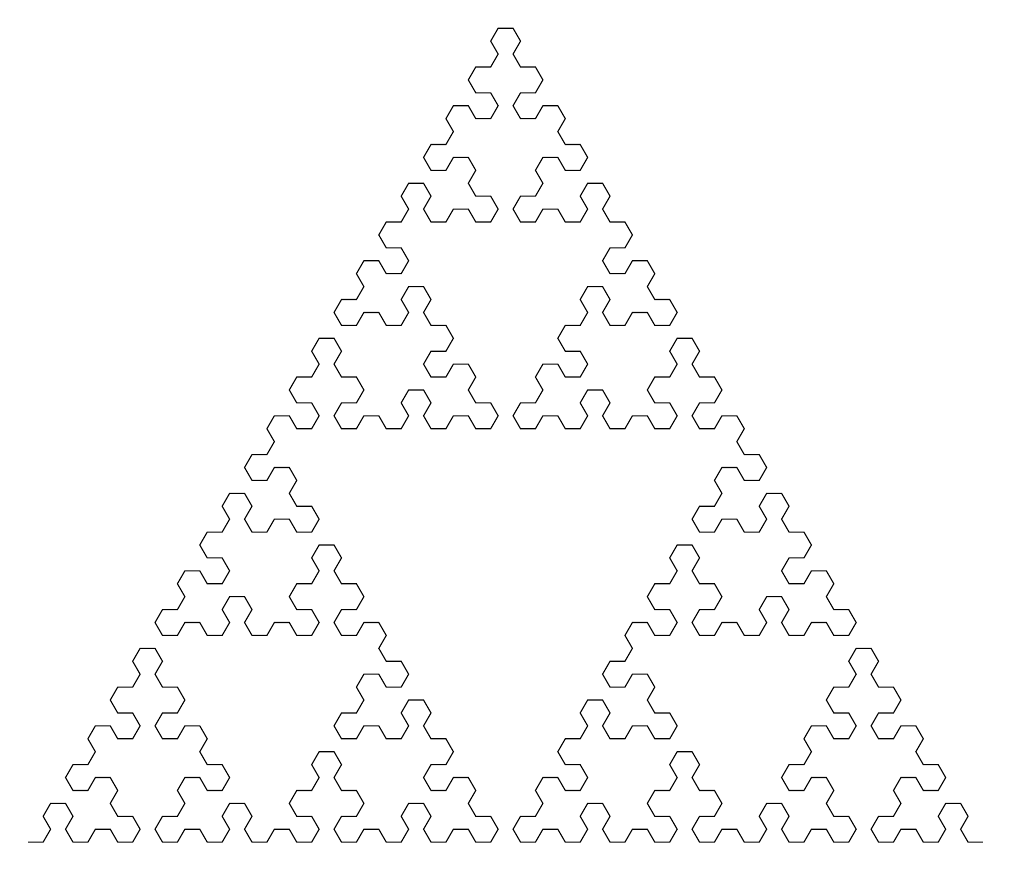
\begin{tikzpicture}
        \draw[] (0, 0) l-system[l-system={Sierpinsky, axiom=X, step=\textwidth/64, order=6, angle=60}];
      \end{tikzpicture}
    \end{minipage}%
    \hfill
    \begin{minipage}{.24\textwidth}
      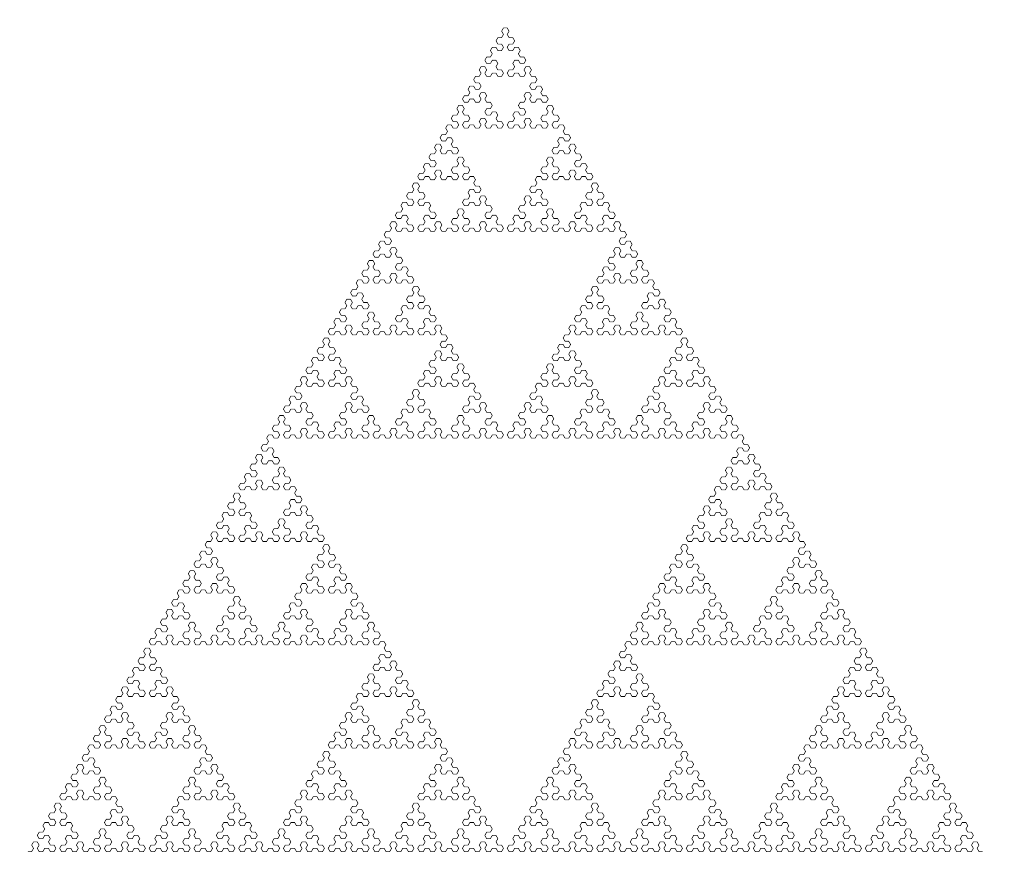
\begin{tikzpicture}
        \draw[very thin] (0, 0) l-system[l-system={Sierpinsky, axiom=X, step=\textwidth/256, order=8, angle=60}];
      \end{tikzpicture}
    \end{minipage}

    \vfill

    \centering
    \textbf{Sierpinski triangle} (dim $\simeq 1.585$)
    
    \vfill
  \end{frame}

  \begin{frame}[t, c, fragile]{}{}
    \vfill
    \centering

    \Large
    \textbf{von Koch snowflake}

    \bigskip

    \large
    \textbf{\color{gray} A self-similar fractal}

    \vfill
  \end{frame}

}


\begin{frame}[t, c]{von Koch snowflake}{}
  \vfill
  %\large

  \begin{minipage}{.28\textwidth}
    \centering
    \begin{tikzpicture}
      \draw[thin] (0, 0) l-system[l-system={Koch curve, axiom=X--X--X, step=\textwidth/81, order=4, angle=60}];
    \end{tikzpicture}
  \end{minipage}%
  \hfill
  \begin{minipage}{.68\textwidth}
    \emph{On a continuous curve without tangents, constructible from elementary geometry}.
    \begin{flushright}
      Helge von Koch, \emph{Ark. Mat. Astron. Fys.}, 1904.
    \end{flushright}
  \end{minipage}

  \vfill
\end{frame}

\begin{frame}[t, c]{von Koch snowflake}{}
  \vfill
  \large

  \begin{minipage}{.28\textwidth}
    \centering
    \begin{overprint}
      \onslide<1>
      \begin{tikzpicture}[baseline]
        \draw[thin, black] (0, 0) l-system[l-system={Koch curve, axiom=X--X--X, step=\textwidth/3, order=1, angle=60}];
        \draw[thin] (0, 0) l-system[l-system={Koch curve, axiom=X--X--X, step=\textwidth, order=0, angle=60}];
      \end{tikzpicture}

      \onslide<2>
      \begin{tikzpicture}[baseline]
        \draw[thin] (0, 0) l-system[l-system={Koch curve, axiom=X--X--X, step=\textwidth/3, order=1, angle=60}];
      \end{tikzpicture}

      \onslide<3>
      \begin{tikzpicture}[baseline]
        \draw[thin] (0, 0) l-system[l-system={Koch curve, axiom=X--X--X, step=\textwidth/9, order=2, angle=60}];
      \end{tikzpicture}

      \onslide<4>
      \begin{tikzpicture}[baseline]
        \draw[thin] (0, 0) l-system[l-system={Koch curve, axiom=X--X--X, step=\textwidth/81, order=4, angle=60}];
      \end{tikzpicture}

    \end{overprint}
  \end{minipage}%
  \hfill
  \begin{minipage}{.68\textwidth}

    \begin{overprint}
      \onslide<1>
      \begin{center}
        \underline{\textbf{Iteration n°0}}
      \end{center}
      
      \bigskip
      
      \begin{tabular}{lr}
        Number of segment & $N_0 = 3$ \\
        \\
        Length of each segment & $L_0 = 1$ \\
        \\
        Perimeter & $P_0 = 3$
      \end{tabular}

      \onslide<2>
      \begin{center}
        \underline{\textbf{Iteration n°1}}
      \end{center}
      
      \bigskip
      
      \begin{tabular}{lr}
        Number of segment & $N_1 = 3 \times 4$ \\
        \\
        Length of each segment & $L_1 = \dfrac{1}{3}$ \\
        \\
        Perimeter & $P_1 = 3 \times \dfrac{4}{3}$
      \end{tabular}


      \onslide<3>
      \begin{center}
        \underline{\textbf{Iteration n°2}}
      \end{center}
      
      \bigskip
      
      \begin{tabular}{lr}
        Number of segment & $N_2 = 3 \times 4^2$ \\
        \\
        Length of each segment & $L_2 = \dfrac{1}{3^2}$ \\
        \\
        Perimeter & $P_2 = 3 \times \left( \dfrac{4}{3} \right)^2$
      \end{tabular}

      \onslide<4>
      \begin{center}
        \underline{\textbf{Iteration n°$n$}}
      \end{center}
      
      \bigskip
      
      \begin{tabular}{lr}
        Number of segment & $N_n = 3 \times 4^n$ \\
        \\
        Length of each segment & $L_n = \dfrac{1}{3^n}$ \\
        \\
        Perimeter & $P_n = 3 \times \left( \dfrac{4}{3} \right)^n$
      \end{tabular}

    \end{overprint}
  \end{minipage}

  \vfill
\end{frame}

\begin{frame}[t, c]{von Koch snowflake}{}
  \vfill
  \large

  \begin{minipage}{.28\textwidth}
    \centering
    \begin{tikzpicture}[baseline]
      \draw[thin] (0, 0) l-system[l-system={Koch curve, axiom=X--X--X, step=\textwidth/81, order=4, angle=60}];
    \end{tikzpicture}
  \end{minipage}%
  \hfill
  \begin{minipage}{.68\textwidth}
    \[
    \lim_{n \to \infty} P_n = \lim_{n \to \infty} 3 \times \left( \dfrac{4}{3} \right)^n
    \]
  \end{minipage}

  \vfill

\end{frame}


\begin{frame}[t, c]{von Koch snowflake}{}
  \vfill
  \large

  \begin{minipage}{.28\textwidth}
    \centering
    \begin{overprint}
      \onslide<1>
      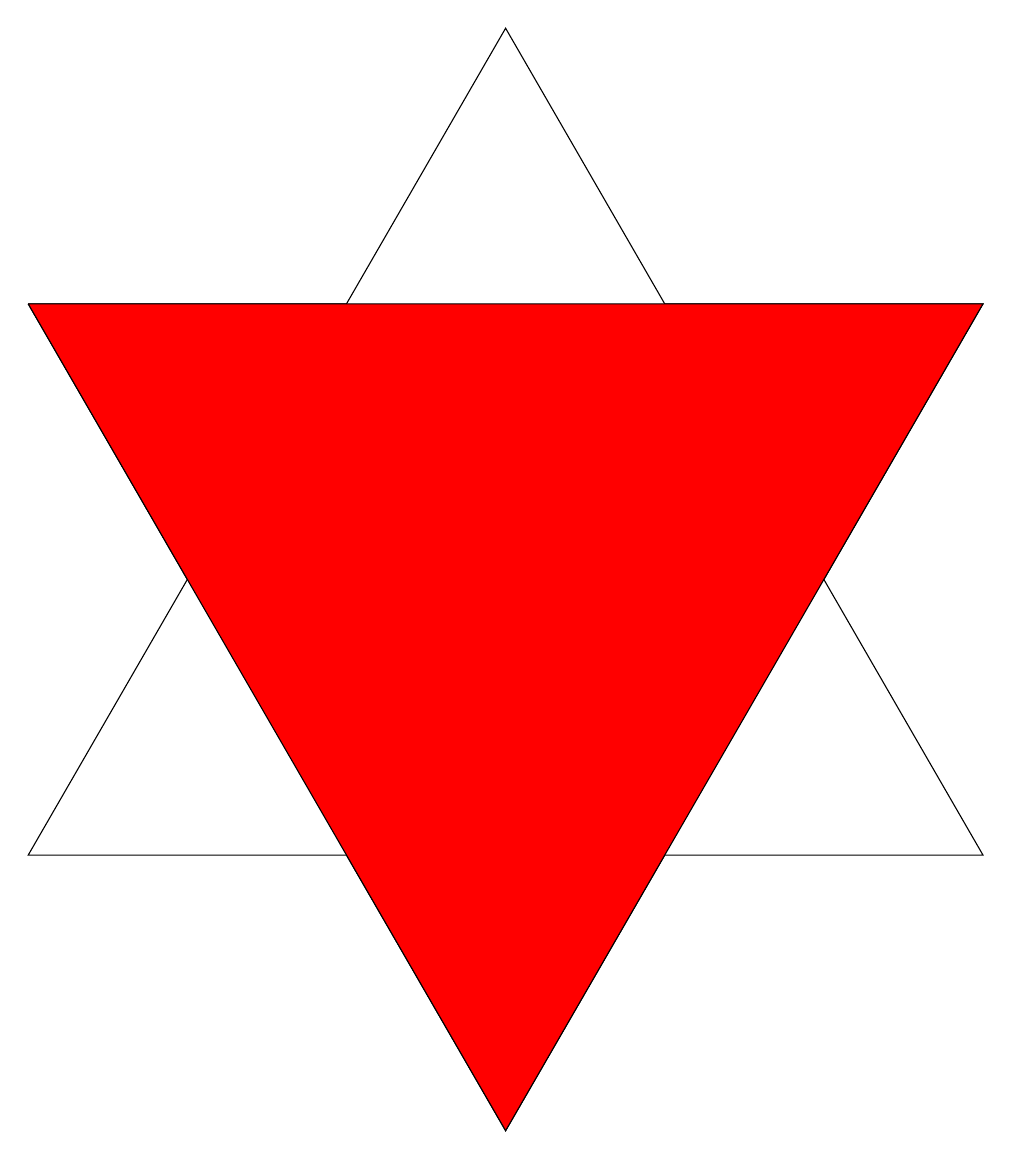
\begin{tikzpicture}[baseline]
        \draw[thin, black] (0, 0) l-system[l-system={Koch curve, axiom=X--X--X, step=\textwidth/3, order=1, angle=60}];
        \draw[thin, fill=red] (0, 0) l-system[l-system={Koch curve, axiom=X--X--X, step=\textwidth, order=0, angle=60}];
      \end{tikzpicture}

      \onslide<2>
      
\begin{tikzpicture}[baseline]
        \draw[thin, fill=red] (0, 0) l-system[l-system={Koch curve, axiom=X--X--X, step=\textwidth/3, order=1, angle=60}];
        \draw[thin, fill=gray] (0, 0) l-system[l-system={Koch curve, axiom=X--X--X, step=\textwidth, order=0, angle=60}];
      \end{tikzpicture}

      \onslide<3>
      
\begin{tikzpicture}[baseline]
        \draw[thin, fill=red] (0, 0) l-system[l-system={Koch curve, axiom=X--X--X, step=\textwidth/9, order=2, angle=60}];
        \draw[thin, fill=gray] (0, 0) l-system[l-system={Koch curve, axiom=X--X--X, step=\textwidth/3, order=1, angle=60}];
      \end{tikzpicture}

      \onslide<4>
      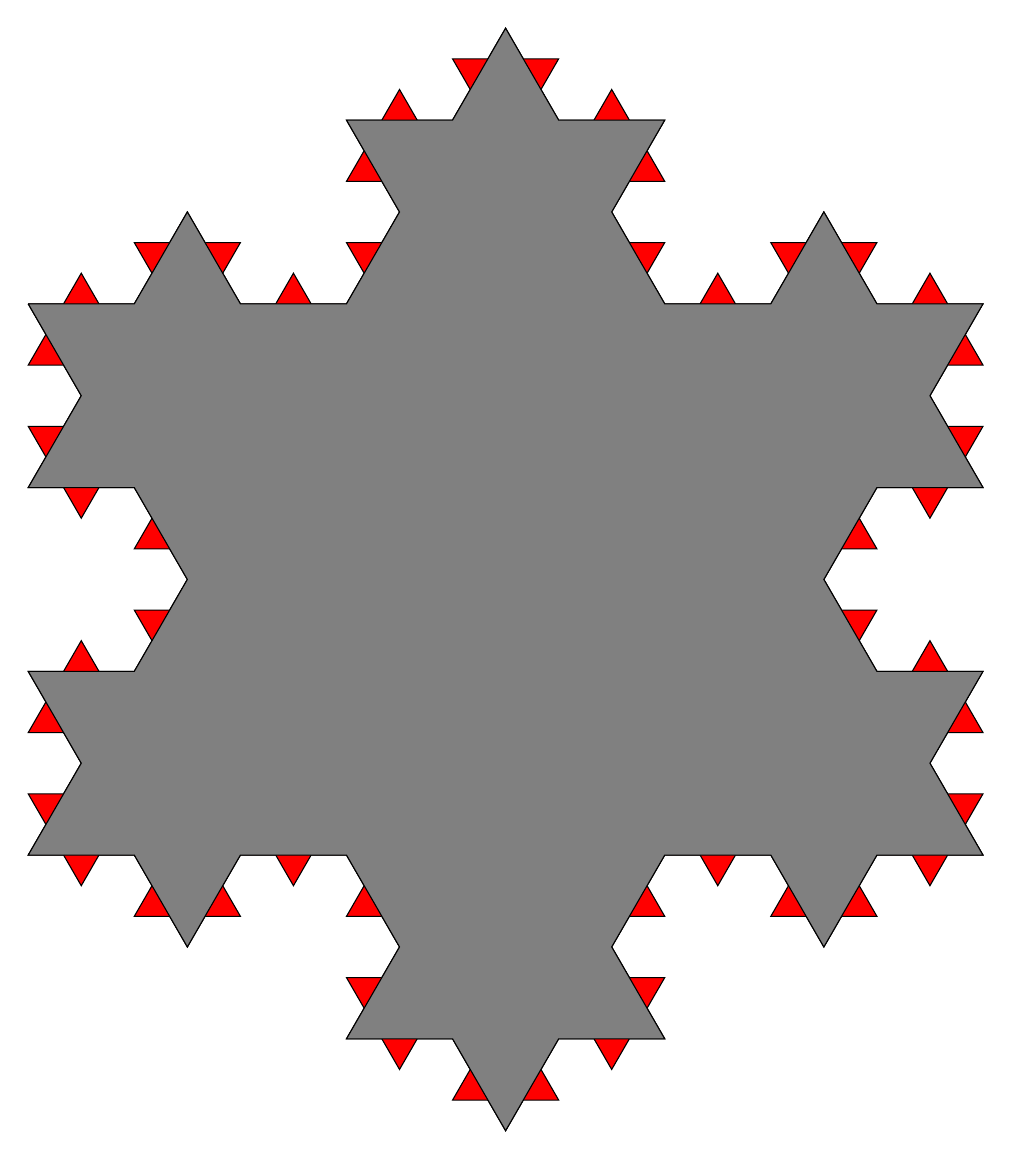
\begin{tikzpicture}[baseline]
        \draw[thin, fill=red] (0, 0) l-system[l-system={Koch curve, axiom=X--X--X, step=\textwidth/27, order=3, angle=60}];
        \draw[thin, fill=gray] (0, 0) l-system[l-system={Koch curve, axiom=X--X--X, step=\textwidth/9, order=2, angle=60}];
      \end{tikzpicture}

    \end{overprint}
  \end{minipage}%
  \hfill
  \begin{minipage}{.68\textwidth}

    \begin{overprint}
      \onslide<1>
      \begin{center}
        \underline{\textbf{Iteration n°0}}
      \end{center}
      
      \bigskip
      
      \begin{tabular}{lr}
        Number of triangles & $T_0 = 1$ \\
        \\
        Surface & $A_0$
      \end{tabular}

      \onslide<2>
      \begin{center}
        \underline{\textbf{Iteration n°1}}
      \end{center}
      
      \bigskip
      
      \begin{tabular}{lr}
        Number of triangles & $T_1 = 3$ \\
        \\
        Surface & $A_1 = A_0 \left( 1 + 3 \times \dfrac{1}{9} \right)$
      \end{tabular}


      \onslide<3>
      \begin{center}
        \underline{\textbf{Iteration n°2}}
      \end{center}
      
      \bigskip
      
      \begin{tabular}{lr}
        Number of triangles & $T_2 = 3 \times 4$ \\
        \\
        Surface & $A_2 = A_1 \left( 1 + \dfrac{3}{4} \times \left( \dfrac{4}{9} \right)^2 \right)$
      \end{tabular}

      \onslide<4>
      \begin{center}
        \underline{\textbf{Iteration n°$n$}}
      \end{center}
      
      \bigskip
      
      \begin{tabular}{lr}
        Number of triangles & $T_n = \dfrac{3}{4} \times 4^n$ \\
        \\
        Surface & $A_n = A_{n-1} \left( 1 + \dfrac{3}{4} \times \left( \dfrac{4}{9} \right)^n \right)$
      \end{tabular}

    \end{overprint}
  \end{minipage}

  \vfill
\end{frame}


\begin{frame}[t, c]{von Koch snowflake}{}
  \vfill
  \large

  \begin{minipage}{.28\textwidth}
    \centering
    
\begin{tikzpicture}[baseline]
      \draw[thin, fill=red] (0, 0) l-system[l-system={Koch curve, axiom=X--X--X, step=\textwidth/81, order=4, angle=60}];
    \end{tikzpicture}
  \end{minipage}%
  \hfill
  \begin{minipage}{.68\textwidth}
    \begin{overprint}
      \onslide<1>
      \[
      \lim_{n \to \infty} A_n = \lim_{n \to \infty} A_{n-1} \left( 1 + \dfrac{3}{4} \left( \dfrac{4}{9} \right)^n \right)
      \]

      \onslide<2>
      \[
      \lim_{n \to \infty} A_n = \lim_{n \to \infty} A_0 \left( 1 + \dfrac{3}{4} \sum_{i=1}^n \left( \dfrac{4}{9} \right)^n \right)
      \]

      \onslide<3>
      \[
      \lim_{n \to \infty} A_n = \lim_{n \to \infty} A_0 \left( 1 + \dfrac{1}{3} \sum_{i=0}^{n-1} \left( \dfrac{4}{9} \right)^n \right)
      \]


      \onslide<4>
      \[
      \lim_{n \to \infty} A_n = \lim_{n \to \infty} \dfrac{A_0}{5} \left( 8 - 3 \left( \dfrac{4}{9} \right)^n \right)
      \]

      \onslide<5>
      \[
      \lim_{n \to \infty} A_n = \dfrac{8}{5} A_0
      \]
    \end{overprint}
  \end{minipage}

  \vfill

\end{frame}


\begin{frame}[t, c]{von Koch snowflake}{}
  \vfill
  \large

  \begin{minipage}{.28\textwidth}
    \centering
    
\begin{tikzpicture}[baseline]
      \draw[thin, fill=red] (0, 0) l-system[l-system={Koch curve, axiom=X--X--X, step=\textwidth/81, order=4, angle=60}];
    \end{tikzpicture}
  \end{minipage}%
  \hfill
  \begin{minipage}{.68\textwidth}
    The snowflake encloses a \textbf{finite area}, but has an \textbf{infinite perimeter}.
    How is this possible ?
  \end{minipage}

  \vfill

\end{frame}

{
  \setbeamercolor{background canvas}{bg=white}
  \setbeamercolor{background canvas}{bg=white}
  \setbeamercolor{normal text}{fg=black}

  \usebeamercolor[fg]{normal text}

  \setbeamercolor{frametitle}{fg=black}
  \setbeamercolor{framesubtitle}{fg=black}
  \setbeamercolor{itemize item}{fg=black}

  \begin{frame}[fragile]{}{}
    \vfill
    \centering
    \Large
    \textbf{\color{black} Hilbert curve}

    \bigskip

    \large
    \textbf{\color{gray} A space-filling curve}
    \vfill
  \end{frame}
}

\begin{frame}[t, c]{Hilbert curve}{}
  \vfill
  \large

  \begin{minipage}{.28\textwidth}
    \begin{overprint}
      \onslide<1>
      \centering
      \begin{tikzpicture}[baseline]
        \draw[thin] (0, 0) l-system[l-system={Hilbert curve, axiom=L, step=\textwidth/4, order=2, angle=90}];
      \end{tikzpicture}

      \onslide<2>
      \centering
      \begin{tikzpicture}[baseline]
        \draw[thin] (0, 0) l-system[l-system={Hilbert curve, axiom=L, step=\textwidth/8, order=3, angle=90}];
      \end{tikzpicture}

      \onslide<3>
      \centering
      \begin{tikzpicture}[baseline]
        \draw[thin] (0, 0) l-system[l-system={Hilbert curve, axiom=L, step=\textwidth/16, order=4, angle=90}];
      \end{tikzpicture}

      \onslide<4>
      \centering
      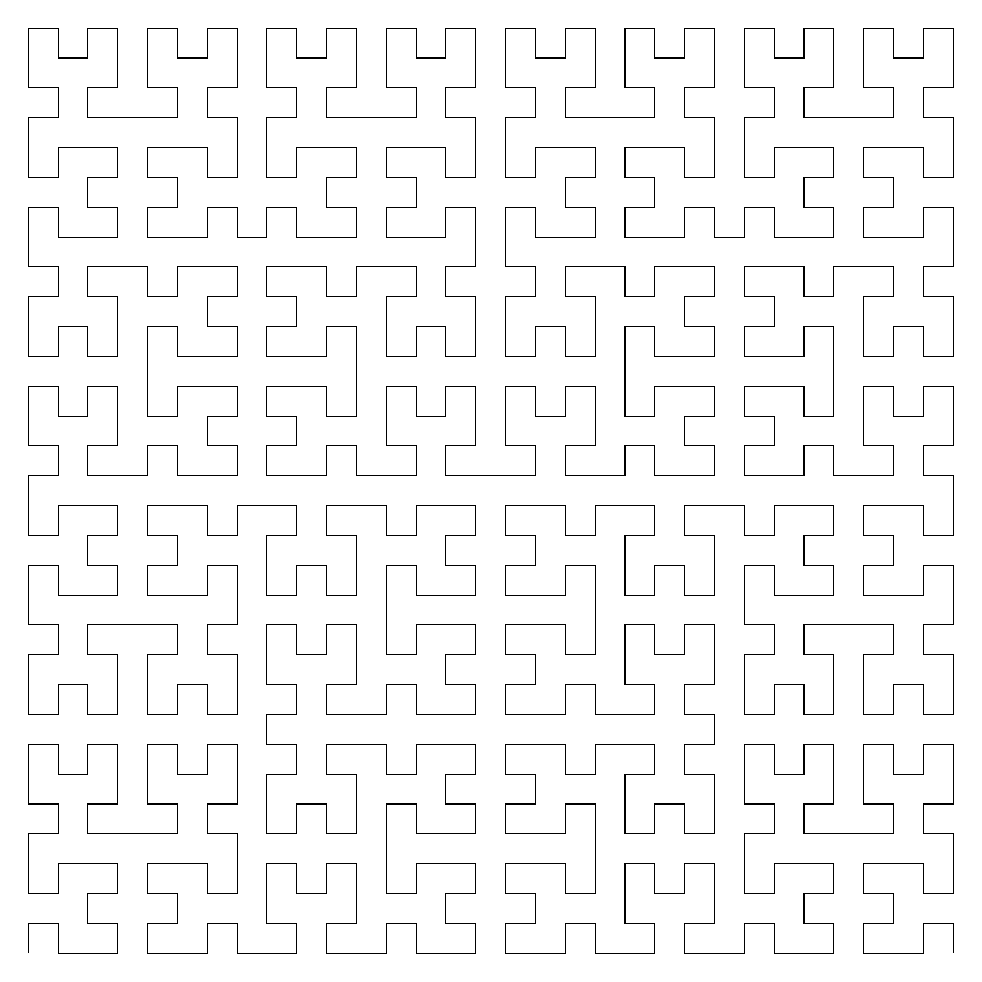
\begin{tikzpicture}[baseline]
        \draw[thin] (0, 0) l-system[l-system={Hilbert curve, axiom=L, step=\textwidth/32, order=5, angle=90}];
      \end{tikzpicture}

      \onslide<5-6>
      \centering
      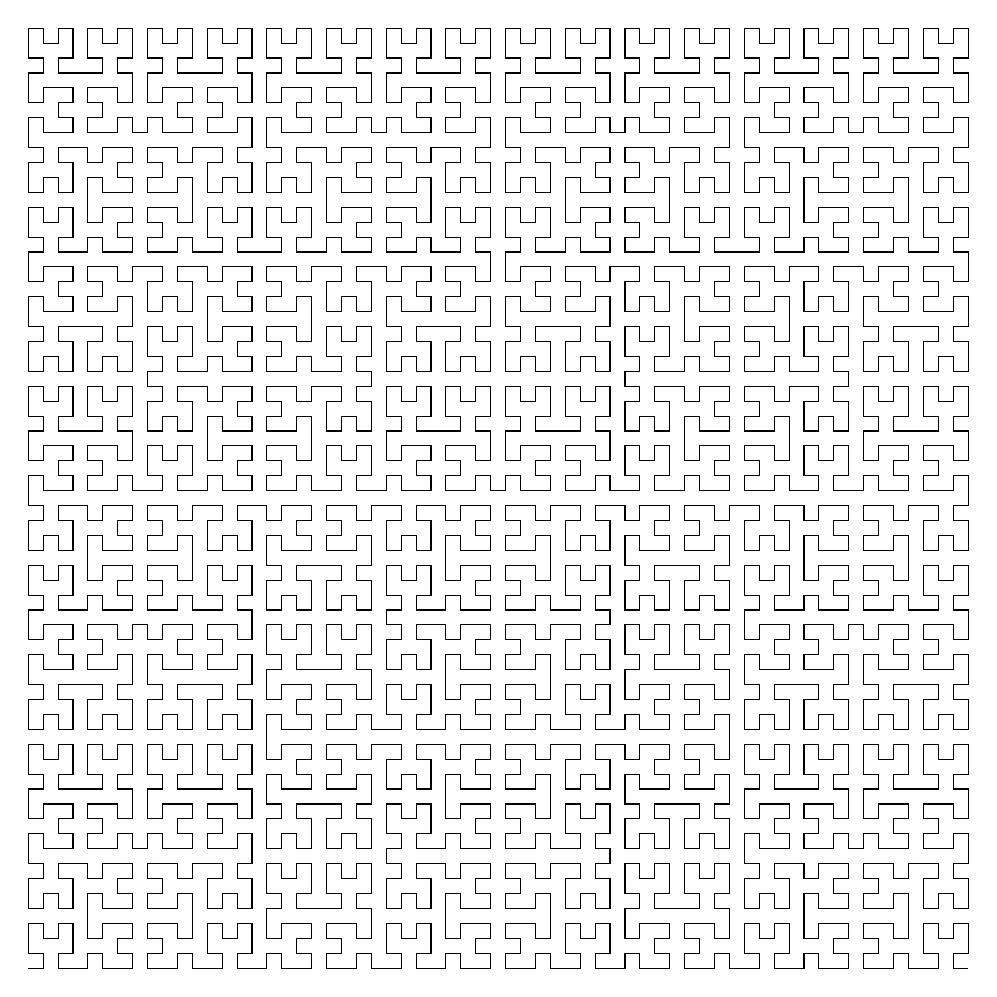
\begin{tikzpicture}[baseline]
        \draw[thin] (0, 0) l-system[l-system={Hilbert curve, axiom=L, step=\textwidth/64, order=6, angle=90}];
      \end{tikzpicture}

    \end{overprint}
  \end{minipage}%
  \hfill
  \begin{minipage}{.68\textwidth}
    \begin{overprint}
      \onslide<1-2>
      \textbf{Hilbert curve} was first described by German mathemacian David Hilbert in 1891.

      \onslide<3-4>
      \[
      L_n = 2^n - \dfrac{1}{2^n}
      \]

      \onslide<5>
      As $n \to \infty$, it has infinite length yet remains enclosed in the unit square.
      It actually goes through every single point of $\mathbb{R}^2$.

      \onslide<6>
      How come the range of a 1D object contains the whole 2D unit square ?
    \end{overprint}
  \end{minipage}

  \vfill
\end{frame}

{
  \setbeamercolor{background canvas}{bg=white}
  \setbeamercolor{background canvas}{bg=white}
  \setbeamercolor{normal text}{fg=black}

  \usebeamercolor[fg]{normal text}

  \setbeamercolor{frametitle}{fg=black}
  \setbeamercolor{framesubtitle}{fg=black}
  \setbeamercolor{itemize item}{fg=black}

  \begin{frame}[fragile]{}{}
    \vfill
    \centering
    \Large
    \textbf{\color{black} Questionning the concept of dimension}

    \bigskip

    \large
    \textbf{\color{gray} The dimension of an object}
    \vfill
  \end{frame}
}

\begin{frame}[t, c]{}{}
  \vfill
  \begin{overprint}
    \onslide<1>
    \centering
    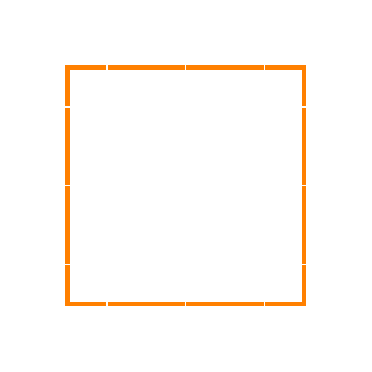
\begin{tikzpicture}
      \draw[ultra thick, orange] (-1.5, -1.5) rectangle (1.5, 1.5);
      
      \foreach \i in {0, ..., 3}{
        \draw[white] (-2, -2 + \i) rectangle (-1, -1 + \i);
        \draw[white] (2, -2 + \i) rectangle (1, -1 + \i);
      }
      
      \foreach \i in {1,2}{
        \draw[white] (-2 + \i, 2) rectangle (-1 + \i, 1);
        \draw[white] (-2 + \i, -2) rectangle (-1 + \i, -1);
      }
      
    \end{tikzpicture}
    
    \onslide<2>
    \centering
    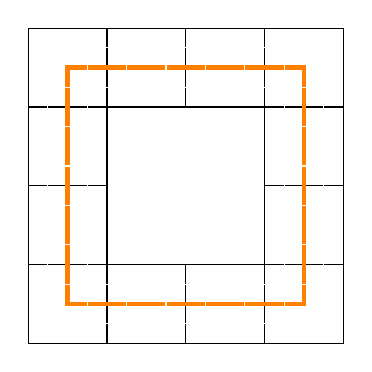
\begin{tikzpicture}
      
      \foreach \i in {0, ..., 3}{
        \draw[black] (-2, -2 + \i) rectangle (-1, -1 + \i);
        \draw[black] (2, -2 + \i) rectangle (1, -1 + \i);
      }
      
      \foreach \i in {1,2}{
        \draw[black] (-2 + \i, 2) rectangle (-1 + \i, 1);
        \draw[black] (-2 + \i, -2) rectangle (-1 + \i, -1);
      }
      
      \draw[ultra thick, orange] (-1.5, -1.5) rectangle (1.5, 1.5);
      
      \foreach \i in {0, ..., 6}{
        \draw[white] (-1.75, -1.75 + 0.5*\i) rectangle (-1.25, -1.25 + 0.5*\i);
        \draw[white] (1.75, -1.75 + 0.5*\i) rectangle (1.25, -1.25 + 0.5*\i);
      }
      
      \foreach \i in {1, ..., 5}{
        \draw[white] (-1.75 + 0.5*\i, -1.75) rectangle (-1.25 + 0.5*\i, -1.25);
        \draw[white] (-1.75 + 0.5*\i, 1.75) rectangle (-1.25 + 0.5*\i, 1.25);
      }
      
    \end{tikzpicture}
    
    \onslide<3>
    \centering
    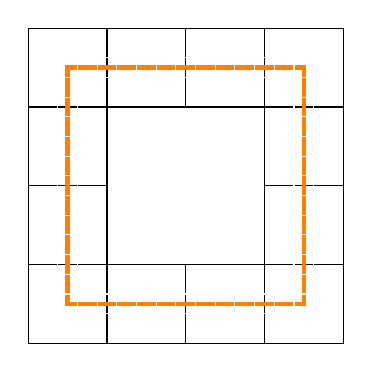
\begin{tikzpicture}
      
      \foreach \i in {0, ..., 3}{
        \draw[black] (-2, -2 + \i) rectangle (-1, -1 + \i);
        \draw[black] (2, -2 + \i) rectangle (1, -1 + \i);
      }
      
      \foreach \i in {1,2}{
        \draw[black] (-2 + \i, 2) rectangle (-1 + \i, 1);
        \draw[black] (-2 + \i, -2) rectangle (-1 + \i, -1);
      }
      
      \draw[ultra thick, orange] (-1.5, -1.5) rectangle (1.5, 1.5);
      
      \foreach \i in {0, ..., 12}{
        \draw[white] (-1.625, -1.625 + 0.25*\i) rectangle (-1.375, -1.375 + 0.25*\i);
        \draw[white] (1.625, -1.625 + 0.25*\i) rectangle (1.375, -1.375 + 0.25*\i);
      }
      
      \foreach \i in {1, ..., 11}{
        \draw[white] (-1.625 + 0.25*\i, -1.625) rectangle (-1.375 + 0.25*\i, -1.375);
        \draw[white] (-1.625 + 0.25*\i, 1.625) rectangle (-1.375 + 0.25*\i, 1.375);
      }
      
    \end{tikzpicture}
    
  \end{overprint}

  \vfill
\end{frame}

\begin{frame}[t, c]{}{}
  \vfill
  \large

  \begin{minipage}{.48\textwidth}
    \centering
    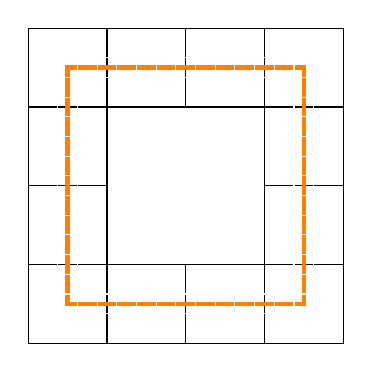
\begin{tikzpicture}
      
      \foreach \i in {0, ..., 3}{
        \draw[black] (-2, -2 + \i) rectangle (-1, -1 + \i);
        \draw[black] (2, -2 + \i) rectangle (1, -1 + \i);
      }
      
      \foreach \i in {1,2}{
        \draw[black] (-2 + \i, 2) rectangle (-1 + \i, 1);
        \draw[black] (-2 + \i, -2) rectangle (-1 + \i, -1);
      }
      
      \draw[ultra thick, orange] (-1.5, -1.5) rectangle (1.5, 1.5);
      
      \foreach \i in {0, ..., 12}{
        \draw[white] (-1.625, -1.625 + 0.25*\i) rectangle (-1.375, -1.375 + 0.25*\i);
        \draw[white] (1.625, -1.625 + 0.25*\i) rectangle (1.375, -1.375 + 0.25*\i);
      }
      
      \foreach \i in {1, ..., 11}{
        \draw[white] (-1.625 + 0.25*\i, -1.625) rectangle (-1.375 + 0.25*\i, -1.375);
        \draw[white] (-1.625 + 0.25*\i, 1.625) rectangle (-1.375 + 0.25*\i, 1.375);
      }
      
    \end{tikzpicture}
  \end{minipage}%
  \hfill
  \begin{minipage}{.48\textwidth}
    \begin{overprint}
      \onslide<1>
      \[
      N \propto \left( \dfrac{1}{\varepsilon} \right)^D
      \]

      \onslide<2>
      \[
      D = -\lim_{\varepsilon \to 0} \dfrac{\log N(\varepsilon)}{\log \varepsilon}
      \]

      \onslide<3>
      \[
      D = 2
      \]
    \end{overprint}
  \end{minipage}

  \vfill
\end{frame}

\begin{frame}[t, c]{}{}
  \vfill
  \large

  \begin{minipage}{.48\textwidth}
    \centering
    \begin{tikzpicture}[baseline]
      \draw[thin] (0, 0) l-system[l-system={Koch curve, axiom=X--X--X, step=\textwidth/81, order=4, angle=60}];
    \end{tikzpicture}
  \end{minipage}%
  \hfill
  \begin{minipage}{.48\textwidth}
    \begin{overprint}
      \onslide<1>
      \[
      D = \dfrac{\log 4}{\log 3}
      \]

      \onslide<2>
      \[
      D \simeq 1.26
      \]
    \end{overprint}
  \end{minipage}

  \vfill
\end{frame}


\begin{frame}[t, c]{}{}
  \vfill
  \large

  \begin{minipage}{.48\textwidth}
    \centering
    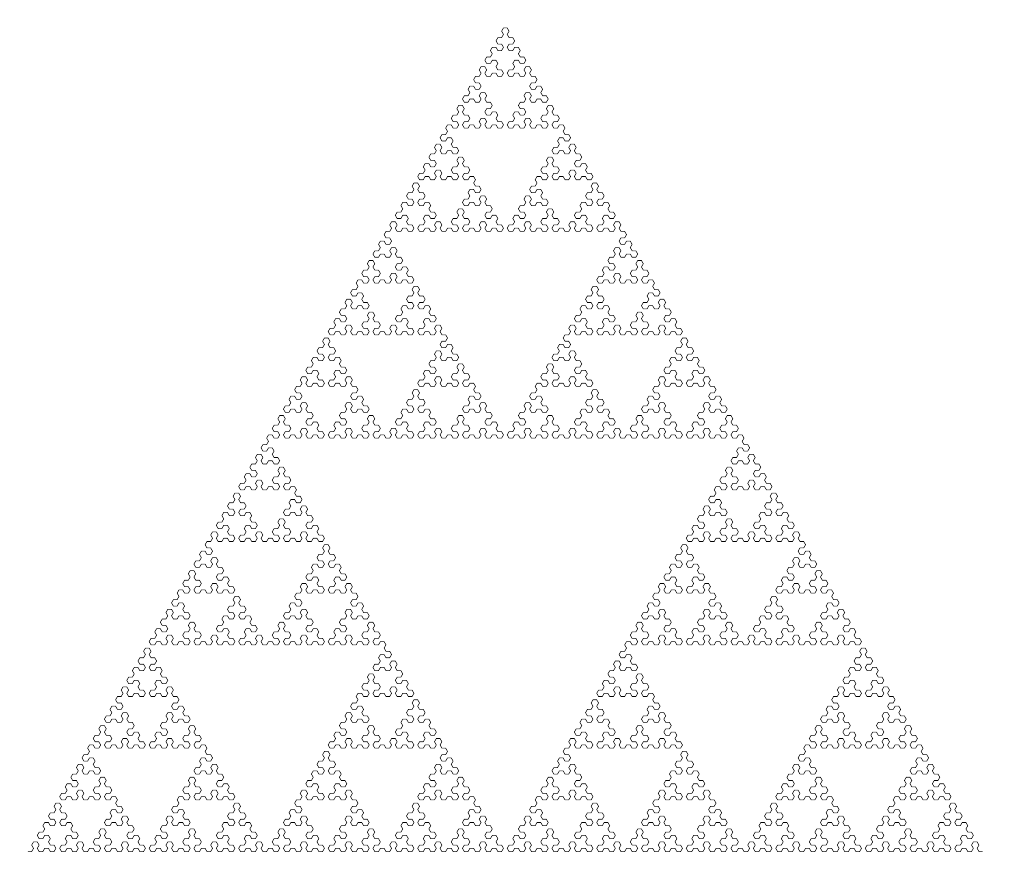
\begin{tikzpicture}[baseline]
      \draw[very thin] (0, 0) l-system[l-system={Sierpinsky, axiom=X, step=\textwidth/256, order=8, angle=60}];
    \end{tikzpicture}
  \end{minipage}%
  \hfill
  \begin{minipage}{.48\textwidth}
    \begin{overprint}
      \onslide<1>
      \[
      D = \dfrac{\log 3}{\log 2}
      \]

      \onslide<2>
      \[
      D \simeq 1.585
      \]
    \end{overprint}
  \end{minipage}

  \vfill
\end{frame}

{
  \setbeamercolor{background canvas}{bg=white}
  \setbeamercolor{background canvas}{bg=white}
  \setbeamercolor{normal text}{fg=black}

  \usebeamercolor[fg]{normal text}

  \setbeamercolor{frametitle}{fg=black}
  \setbeamercolor{framesubtitle}{fg=black}
  \setbeamercolor{itemize item}{fg=black}

  \begin{frame}[fragile]{}{}
    \vfill
    \centering
    \Large
    \textbf{\color{black} Fractals in Nature and Engineering}

    \bigskip

    \large
    \textbf{\color{gray} Some illustrations}
    \vfill
  \end{frame}
}

\begin{frame}[t, c]{In Nature}{}
  \vfill
  \large
  \begin{minipage}{.48\textwidth}
    \centering
    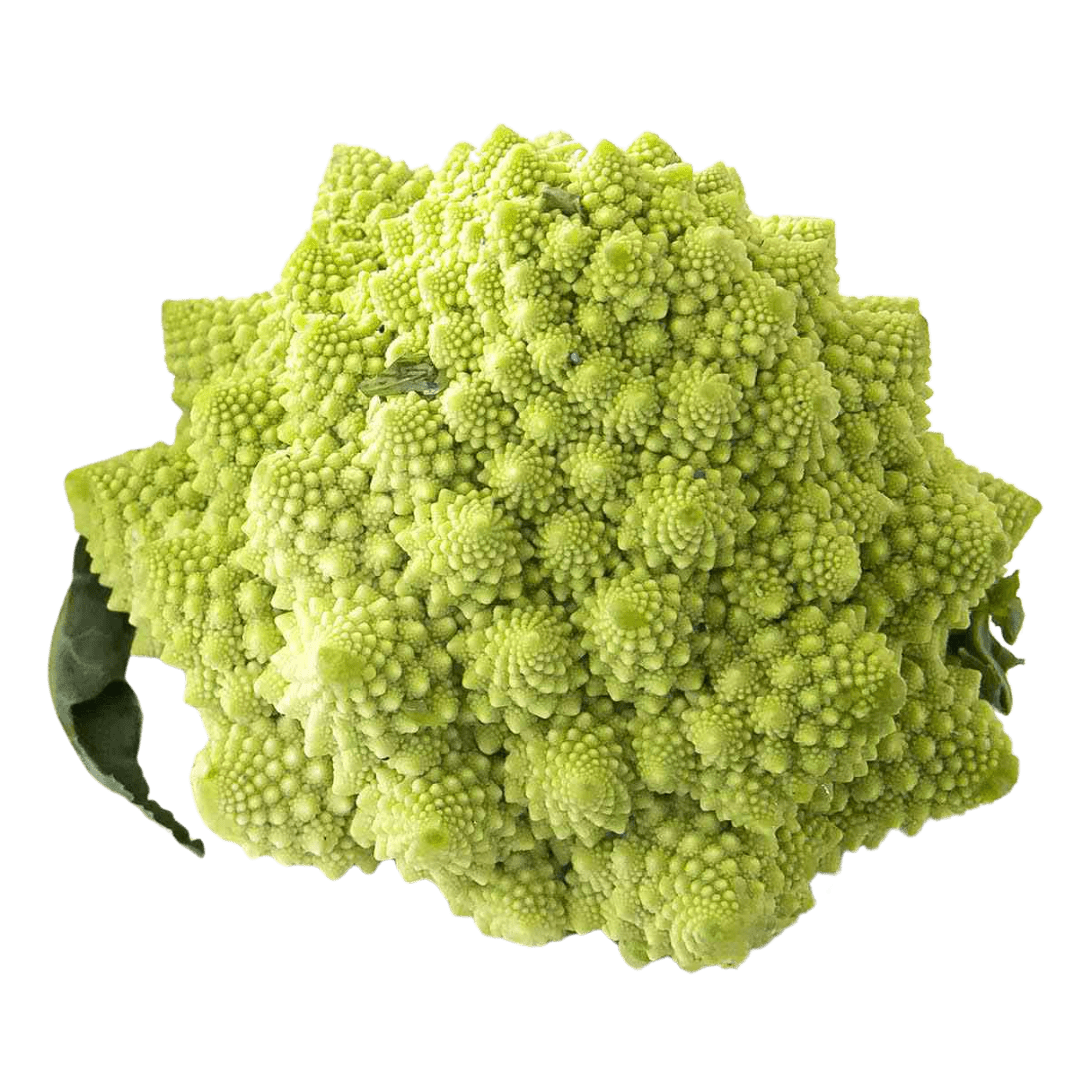
\includegraphics[width=\textwidth]{romanesco}
  \end{minipage}%
  \hfill
  \begin{minipage}{.48\textwidth}
    \begin{overprint}
      \onslide<1>
      A power-law relationship exists between the rate at which the plant grows and the rate at which it produces buds.

      \onslide<2>
      Spirals are closely related to the Fibonacci sequence and the golden ratio.

    \end{overprint}
  \end{minipage}

  \vfill
\end{frame}

\begin{frame}[t, c]{In Nature}{}
  \vfill

  \centering
  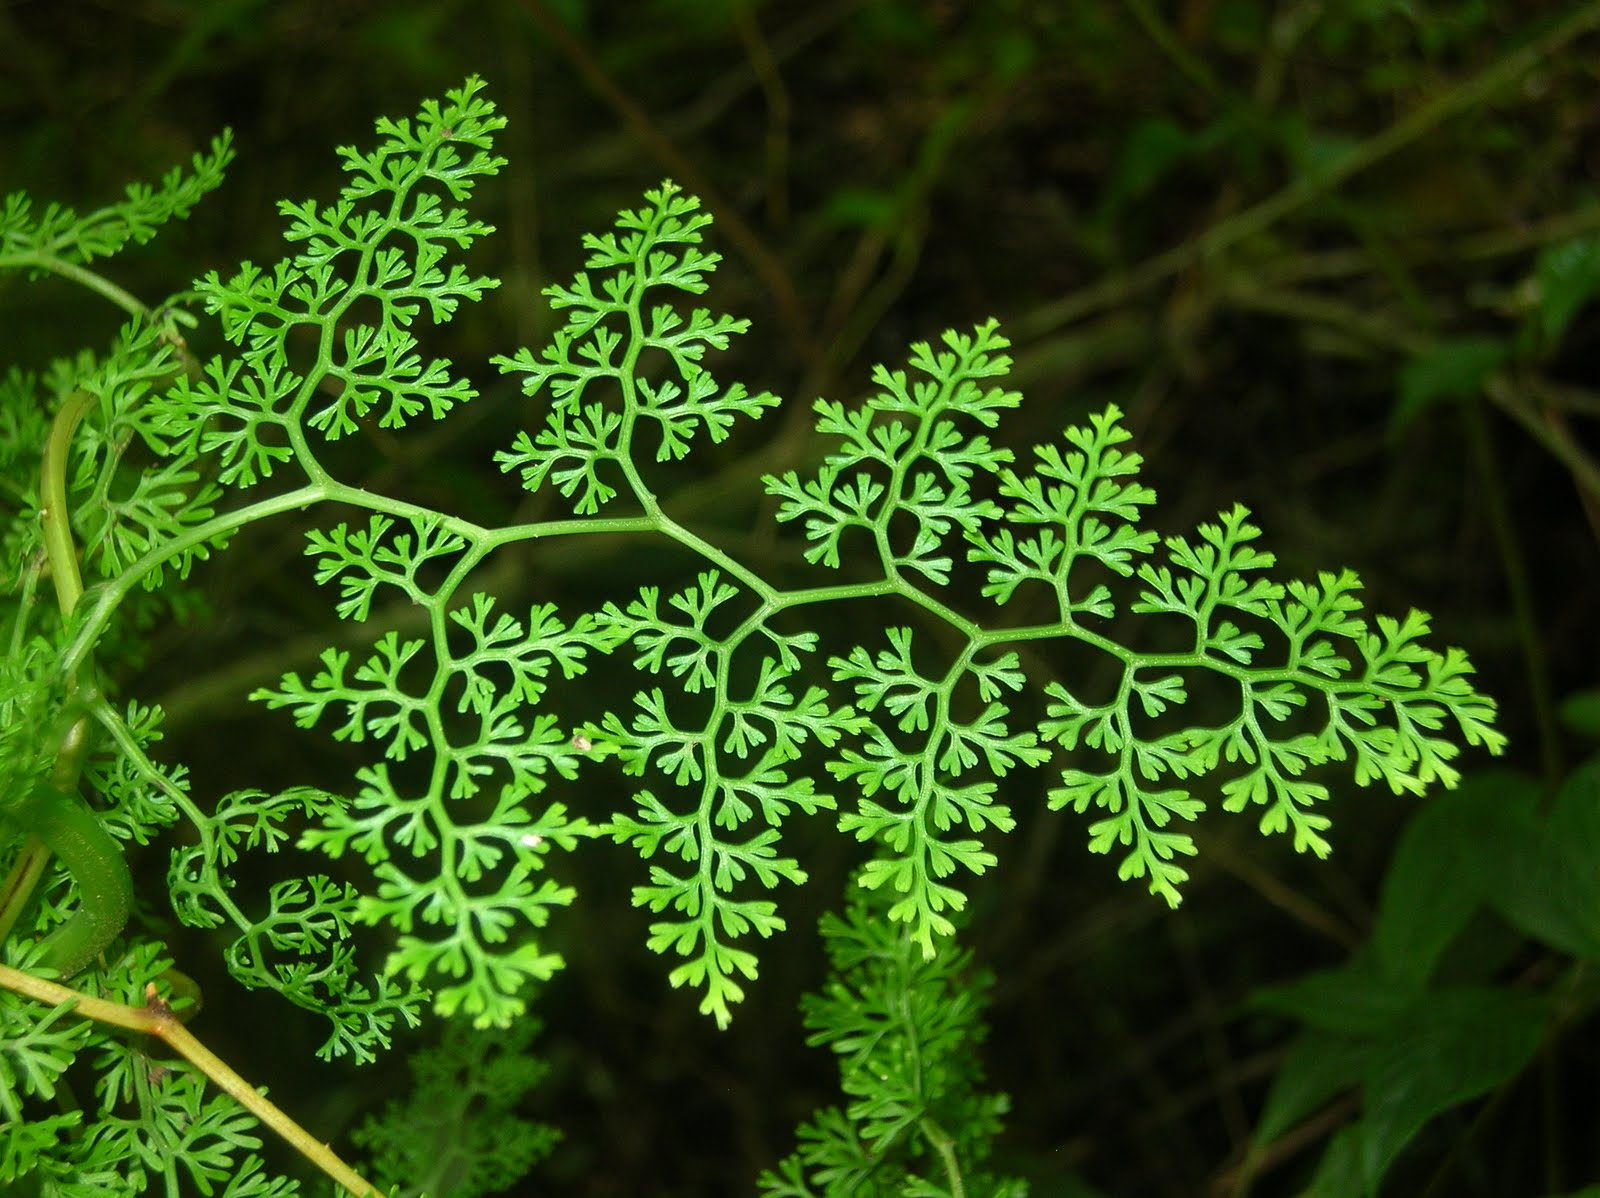
\includegraphics[width=.5\textwidth]{fougere}

  \vfill
\end{frame}

\begin{frame}[t, c]{In Nature}{}
  \vfill
  \large

  \begin{minipage}{.48\textwidth}
    \centering
    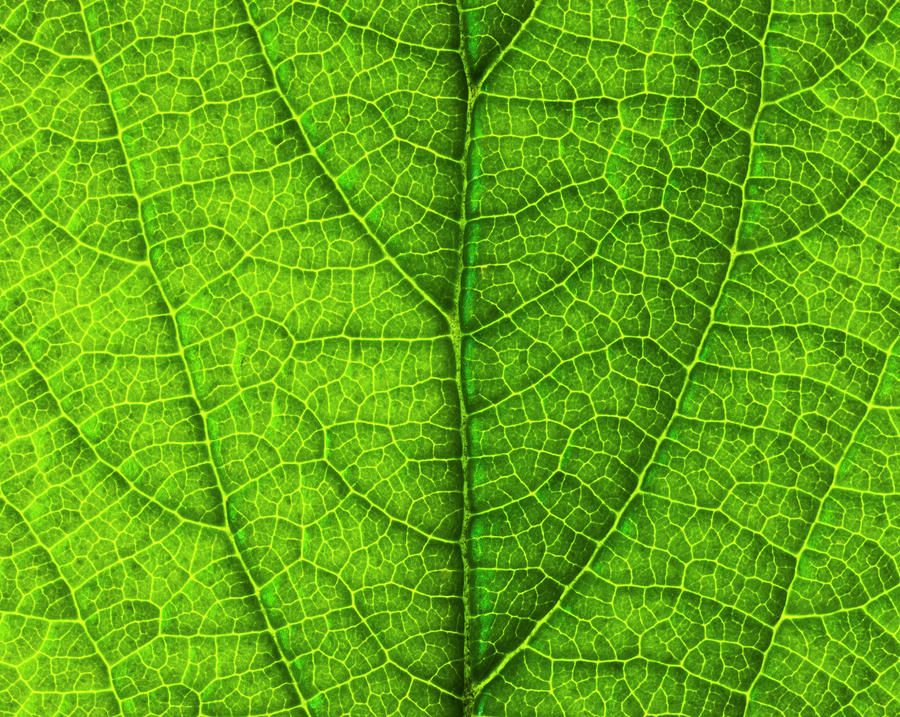
\includegraphics[width=\textwidth]{leaf}
  \end{minipage}%
  \hfill
  \begin{minipage}{.48\textwidth}
    Fractal structure of the veins network ensures an almost optimal coverage the surface of the leaf.
  \end{minipage}

  \vfill
\end{frame}

\begin{frame}[t, c]{In Nature}{}
  \vfill
  \large

  \begin{minipage}{.48\textwidth}
    \centering
    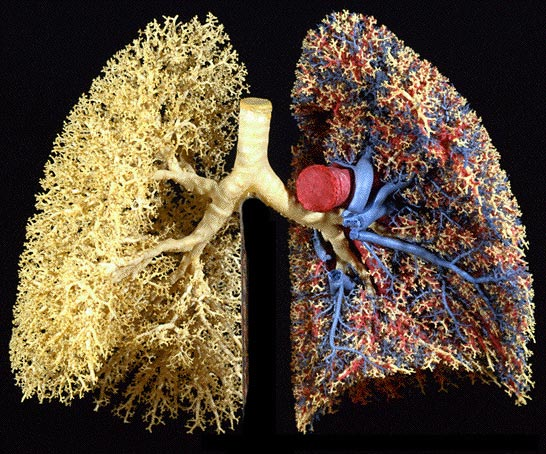
\includegraphics[width=\textwidth]{poumons}
  \end{minipage}%
  \hfill
  \begin{minipage}{.48\textwidth}
    The fractal structure of the lungs encloses a extremely large exchange surface in an otherwise fairly small volume.
  \end{minipage}

  \vfill
\end{frame}

\begin{frame}[t, c]{In Nature}{}
  \vfill
  \centering

  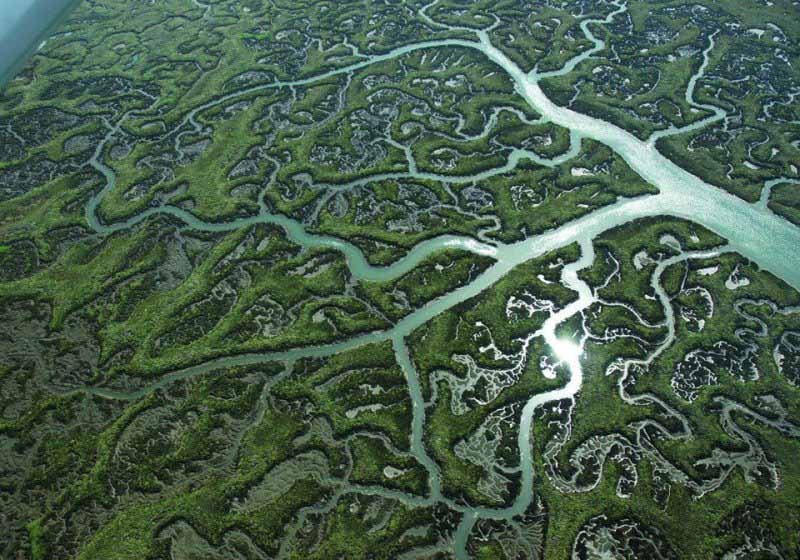
\includegraphics[width=.666\textwidth]{river}

  \vfill
\end{frame}

\begin{frame}[t, c]{In Engineering}{Material science}
  \vfill
  \large

  \begin{minipage}{.48\textwidth}
    \centering
    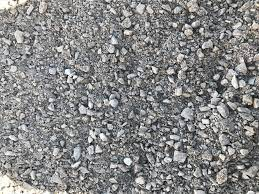
\includegraphics[width=\textwidth]{asphalt}
  \end{minipage}%
  \hfill
  \begin{minipage}{.48\textwidth}
    The fractal nature of aggregates used for asphalt directly impact its mechanical properties.
  \end{minipage}

  \vfill
\end{frame}


\begin{frame}[t, c]{In Engineering}{Thermal systems}
  \vfill
  \large

  \begin{minipage}{.48\textwidth}
    \centering
    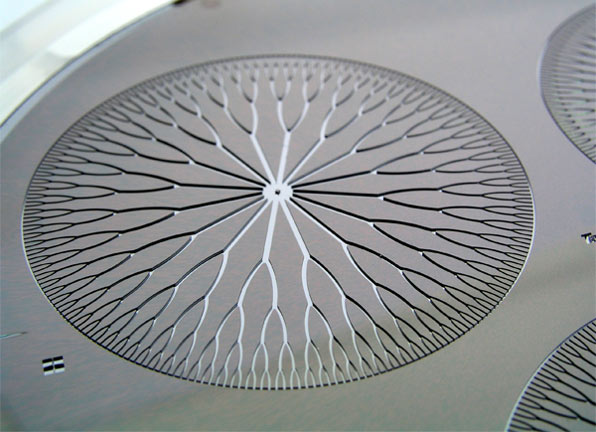
\includegraphics[width=\textwidth]{heat_exchange}
  \end{minipage}%
  \hfill
  \begin{minipage}{.48\textwidth}
    Heat exchanges with self-similar structures have increased efficiency.
  \end{minipage}

  \vfill
\end{frame}

\begin{frame}[t, c]{In Engineering}{Urbanism}
  \centering
  \vfill

  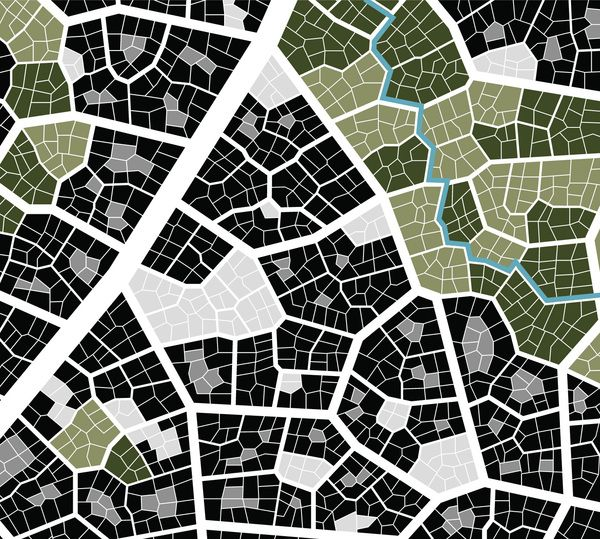
\includegraphics[width=.5\textwidth]{city_planning}

  \vfill
\end{frame}


\begin{frame}[t, c]{In Engineering}{Computer graphics}
  \centering
  \vfill

  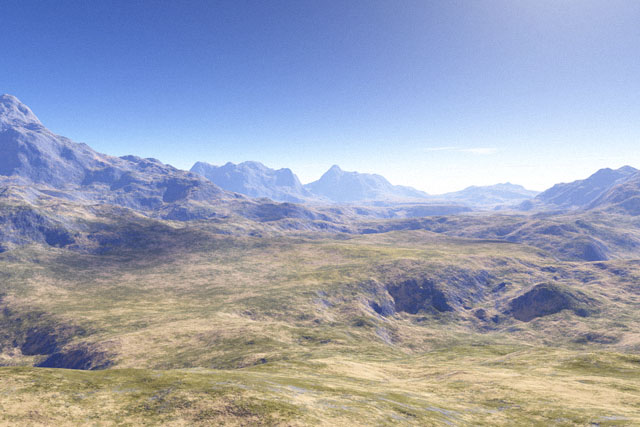
\includegraphics[width=.666\textwidth]{fractal_landscape}

  \vfill
\end{frame}


{
  \setbeamercolor{background canvas}{bg=white}
  \setbeamercolor{background canvas}{bg=white}
  \setbeamercolor{normal text}{fg=black}

  \usebeamercolor[fg]{normal text}

  \setbeamercolor{frametitle}{fg=black}
  \setbeamercolor{framesubtitle}{fg=black}
  \setbeamercolor{itemize item}{fg=black}

  \begin{frame}[fragile]{}{}
    \vfill
    \centering
    \Large
    \textbf{\color{black} Fractal emergence in simple simulations}

    \bigskip

    \large
    \textbf{\color{gray} Some examples}
    \vfill
  \end{frame}
}

\begin{frame}[t, c]{Diffusion-Limited Aggregation}{}
  \vfill
  \large

  \begin{minipage}{.48\textwidth}
    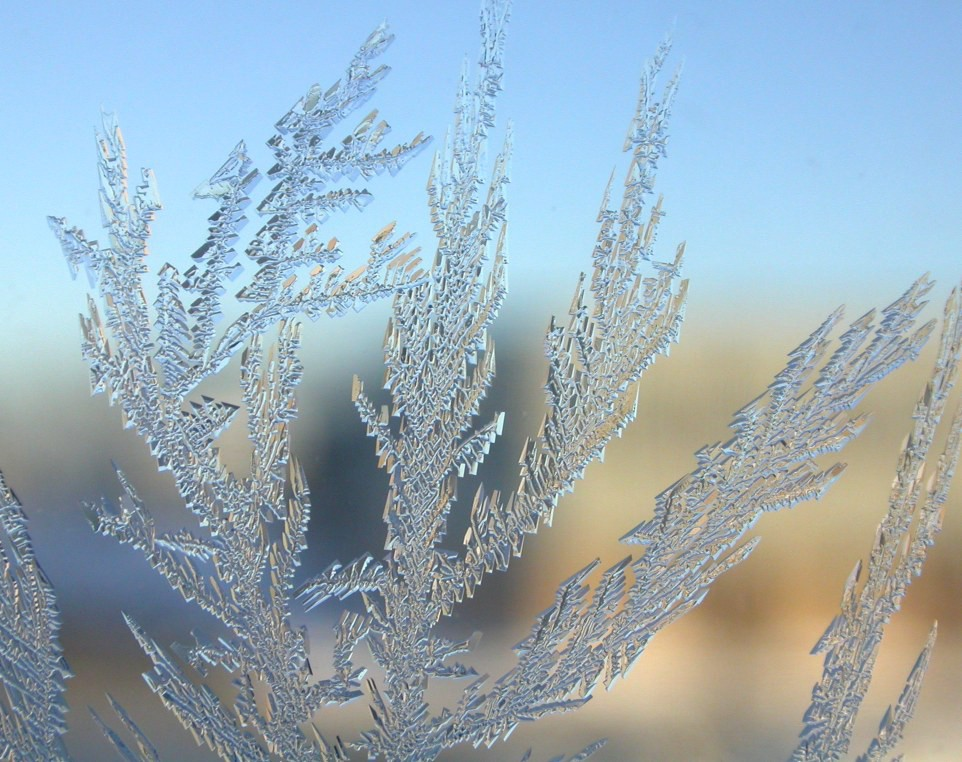
\includegraphics[width=\textwidth]{ice_dla}
  \end{minipage}%
  \hfill
  \begin{minipage}{.48\textwidth}
    Numerous natural phenomena exhibit fractal scaling laws.
    Some of these can be captured by simple \textbf{\alert{Diffusion-Limited Aggregation}} models.
  \end{minipage}

  \vfill
\end{frame}

{
  \setbeamercolor{background canvas}{bg=white}
  \setbeamercolor{background canvas}{bg=white}
  \setbeamercolor{normal text}{fg=black}

  \usebeamercolor[fg]{normal text}

  \setbeamercolor{frametitle}{fg=black}
  \setbeamercolor{framesubtitle}{fg=black}
  \setbeamercolor{itemize item}{fg=black}

  \begin{frame}[fragile]{}{}
    \vfill
    \centering

    \begin{minipage}{.32\textwidth}
      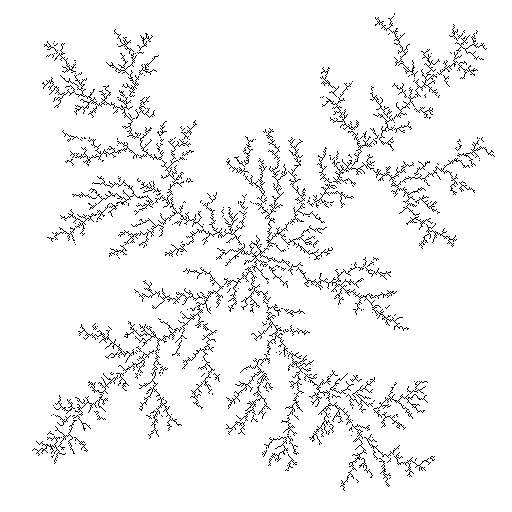
\includegraphics[width=\textwidth]{DLA_1}
    \end{minipage}%
    \hfill
    \begin{minipage}{.32\textwidth}
      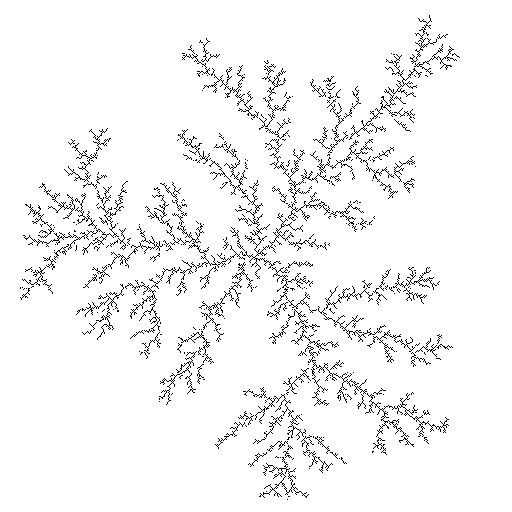
\includegraphics[width=\textwidth]{DLA_2}
    \end{minipage}%
    \hfill
    \begin{minipage}{.32\textwidth}
      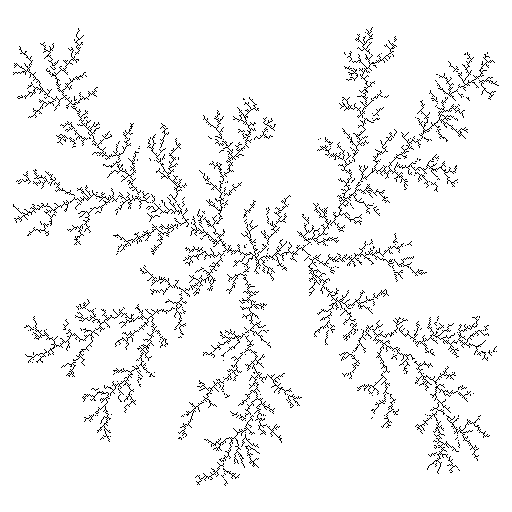
\includegraphics[width=\textwidth]{DLA_3}
    \end{minipage}

    \vfill
  \end{frame}
}

\begin{frame}[t, c]{Diffusion-Limited Aggregation}{}
  \vfill
  \large

  \begin{minipage}{.28\textwidth}
    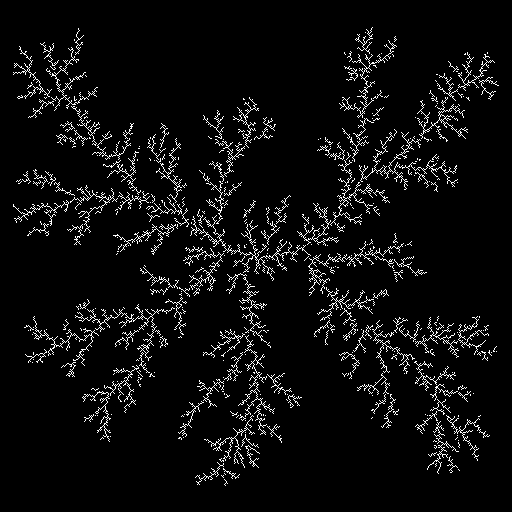
\includegraphics[width=\textwidth]{DLA_4}
  \end{minipage}%
  \hfill
  \begin{minipage}{.68\textwidth}
    \centering
    \begin{tikzpicture}[>=stealth]
      \begin{axis}[
          xmin=0, xmax=400,
          ymin=0, ymax=15000,
          xlabel={Radius $r$}, ylabel={Mass $M(r)$},
          width=\textwidth,
          height=.6\textheight,
          axis lines = middle,
          axis line style = {->},
          x label style={at={(axis description cs:0.5, 0)}, anchor=north},
          y label style={at={(axis description cs:0, 0.5)}, anchor=south, rotate=90},
          ytick style={draw=none},
          yticklabels=\empty,
          scaled y ticks = false,
          xtick style={draw=none},
          xticklabels=\empty,
        ]
        
        \addplot[only marks, orange, mark size=1pt] table[x=x, y=y]{data/fractal_scaling.dat};
        
        \addplot[domain=0:300, dashed] {0.39167*x^2 + 58.4327};
        
        \node[] (source) at (axis cs: 100, 4034) {};
        \node[anchor=south] (destination) at (axis cs:75, 12000) {\small $M(r) \propto r^2$};
        \draw[->] (destination) -- (source);
        
      \end{axis}
    \end{tikzpicture}
  \end{minipage}
  
  \vfill
\end{frame}

\begin{frame}[t, c]{Diffusion-Limited Aggregation}{}
  \vfill
  \large

  \begin{minipage}{.28\textwidth}
    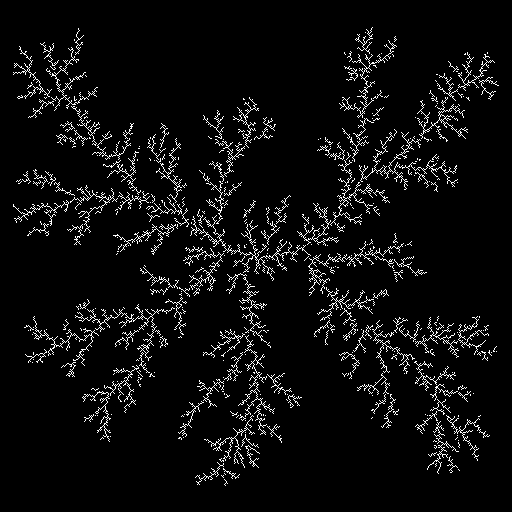
\includegraphics[width=\textwidth]{DLA_4}
  \end{minipage}%
  \hfill
  \begin{minipage}{.68\textwidth}
    \centering

    \[
    M(r) \propto r^{1.71}
    \]

  \end{minipage}
  
  \vfill
\end{frame}

\begin{frame}
  \vfill
  \centering

  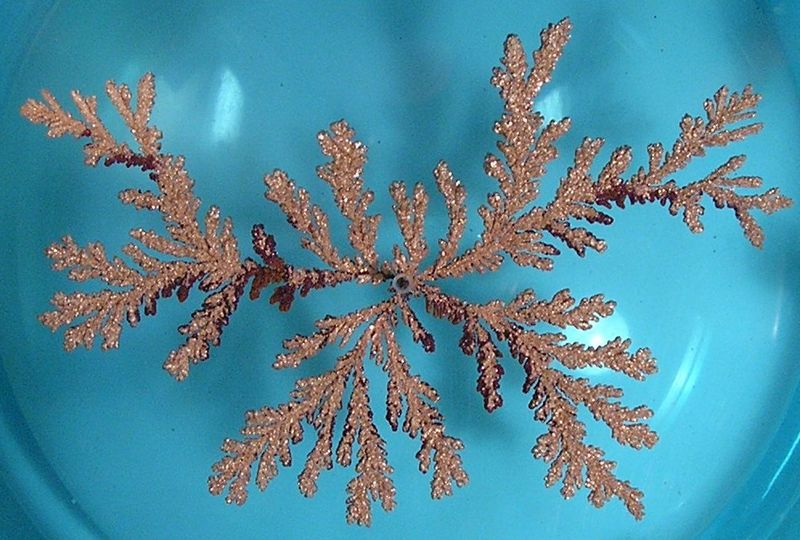
\includegraphics[width=.75\textwidth]{dla_cluster}

  \vfill
\end{frame}

\begin{frame}
  \vfill
  \centering

  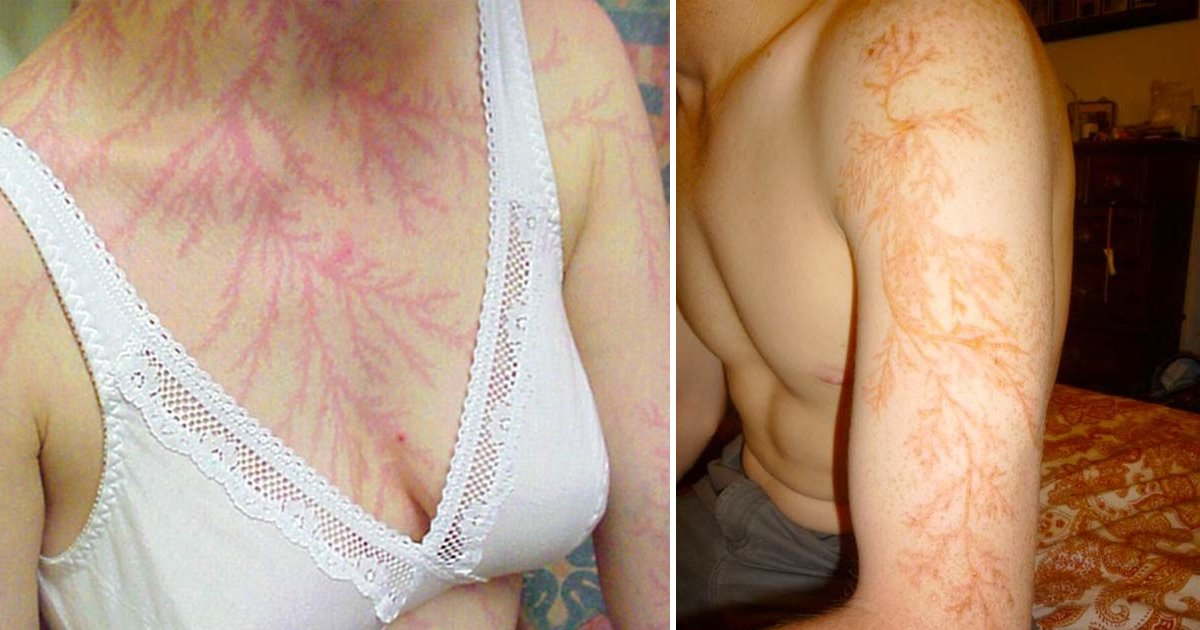
\includegraphics[width=.75\textwidth]{lichtenberg}

  \vfill
\end{frame}

{
  \setbeamercolor{background canvas}{bg=white}
  \setbeamercolor{background canvas}{bg=white}
  \setbeamercolor{normal text}{fg=black}

  \usebeamercolor[fg]{normal text}

  \setbeamercolor{frametitle}{fg=black}
  \setbeamercolor{framesubtitle}{fg=black}
  \setbeamercolor{itemize item}{fg=black}

  \begin{frame}[fragile]{}{}
    \vfill
    \centering
    \Large
    \textbf{\color{black} Iterated Fractals Systems}

    \bigskip

    \large
    \textbf{\color{gray} The Chaos Game}
    \vfill
  \end{frame}
}

\begin{frame}[t, c]{}{}
  \vfill
  \large

  \begin{minipage}{.48\textwidth}
    \[
    f_1(x, y)
    =
    \dfrac{1}{2}
    \begin{bmatrix}
      1 & 0 \\ 0 & 1
    \end{bmatrix}
    \begin{bmatrix}
      x \\ y
    \end{bmatrix}
    \]
  \end{minipage}%
  \hfill
  \begin{minipage}{.48\textwidth}
    \[
    f_2(x, y)
    =
    \dfrac{1}{2}
    \begin{bmatrix}
      1 & 0 \\ 0 & 1
    \end{bmatrix}
    \begin{bmatrix}
      x \\ y
    \end{bmatrix}
    +
    \dfrac{1}{2}
    \begin{bmatrix}
      w \\ 0
    \end{bmatrix}
    \]
  \end{minipage}

  \vfill

  \[
  f_3(x, y)
  =
  \dfrac{1}{2}
  \begin{bmatrix}
    1 & 0 \\ 0 & 1
  \end{bmatrix}
  \begin{bmatrix}
    x \\ y
  \end{bmatrix}
  +
  \dfrac{1}{4}
  \begin{bmatrix}
    w \\ 2h
  \end{bmatrix}
  \]

  \vfill
\end{frame}

{
  \setbeamercolor{background canvas}{bg=white}
  \setbeamercolor{background canvas}{bg=white}
  \setbeamercolor{normal text}{fg=black}

  \usebeamercolor[fg]{normal text}

  \setbeamercolor{frametitle}{fg=black}
  \setbeamercolor{framesubtitle}{fg=black}
  \setbeamercolor{itemize item}{fg=black}

  \begin{frame}
    \vfill

    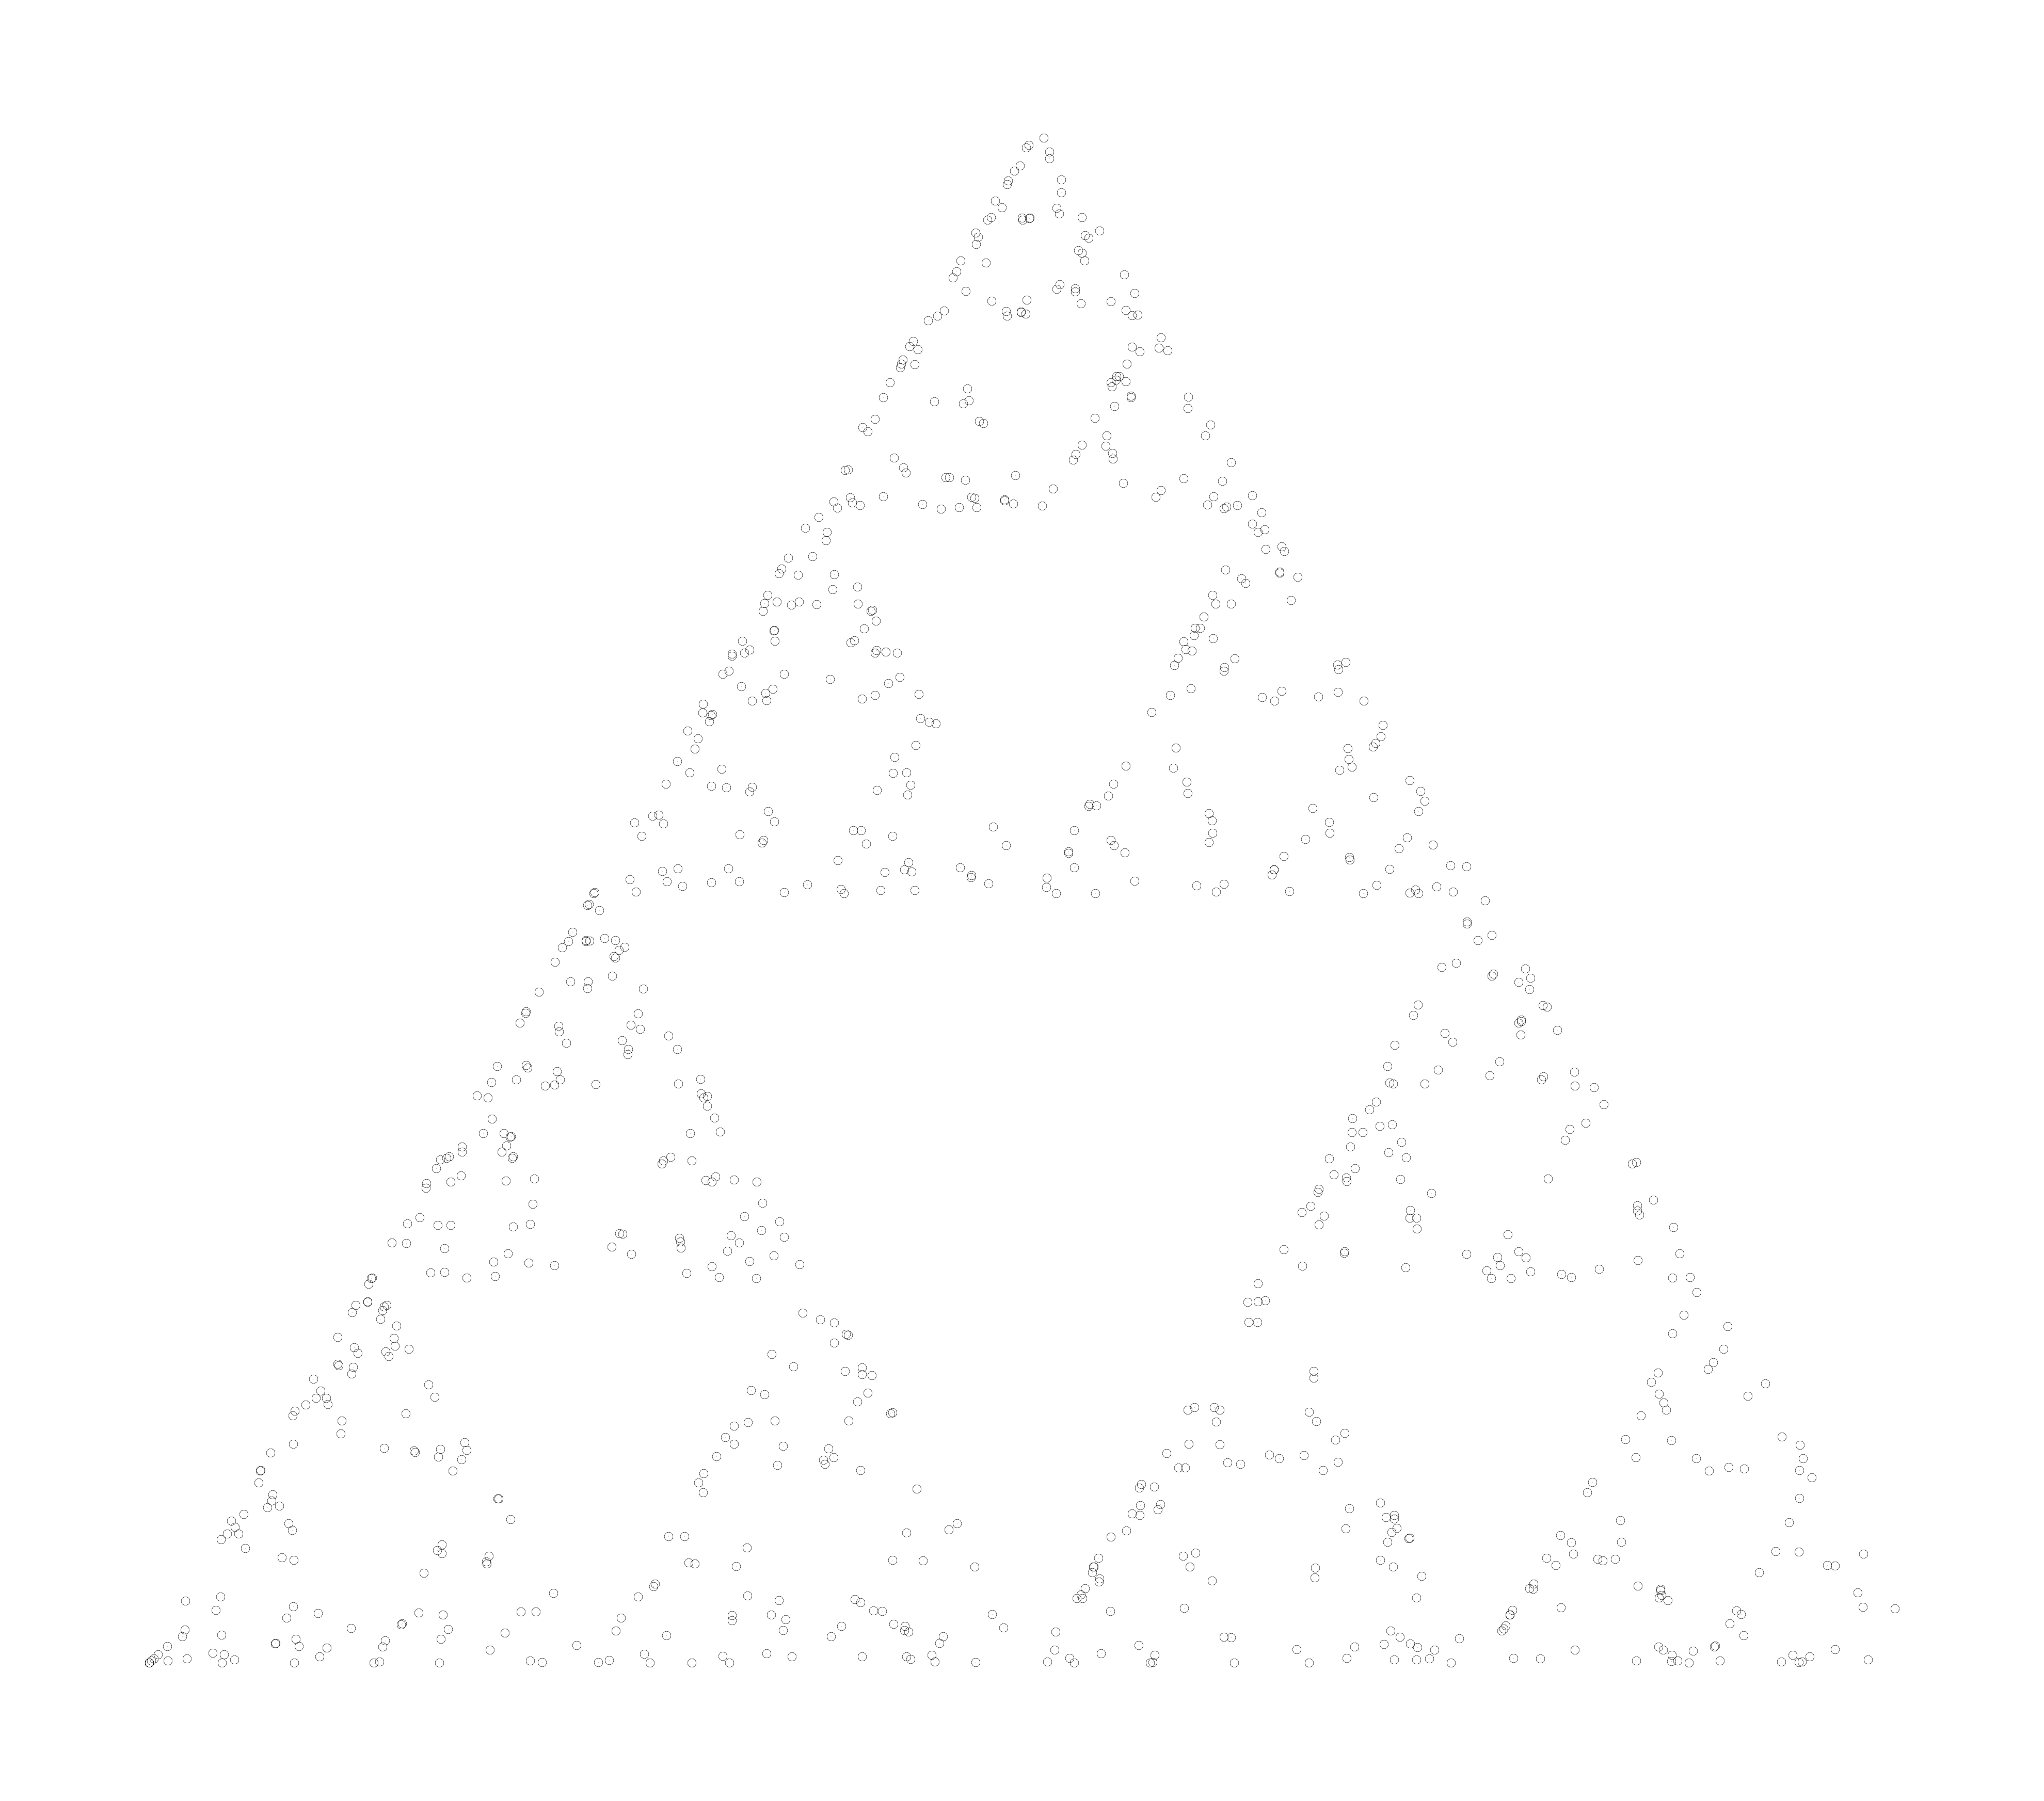
\includegraphics[width=.28\textwidth]{sierpinsky_triangle_1}%
    \hfill
    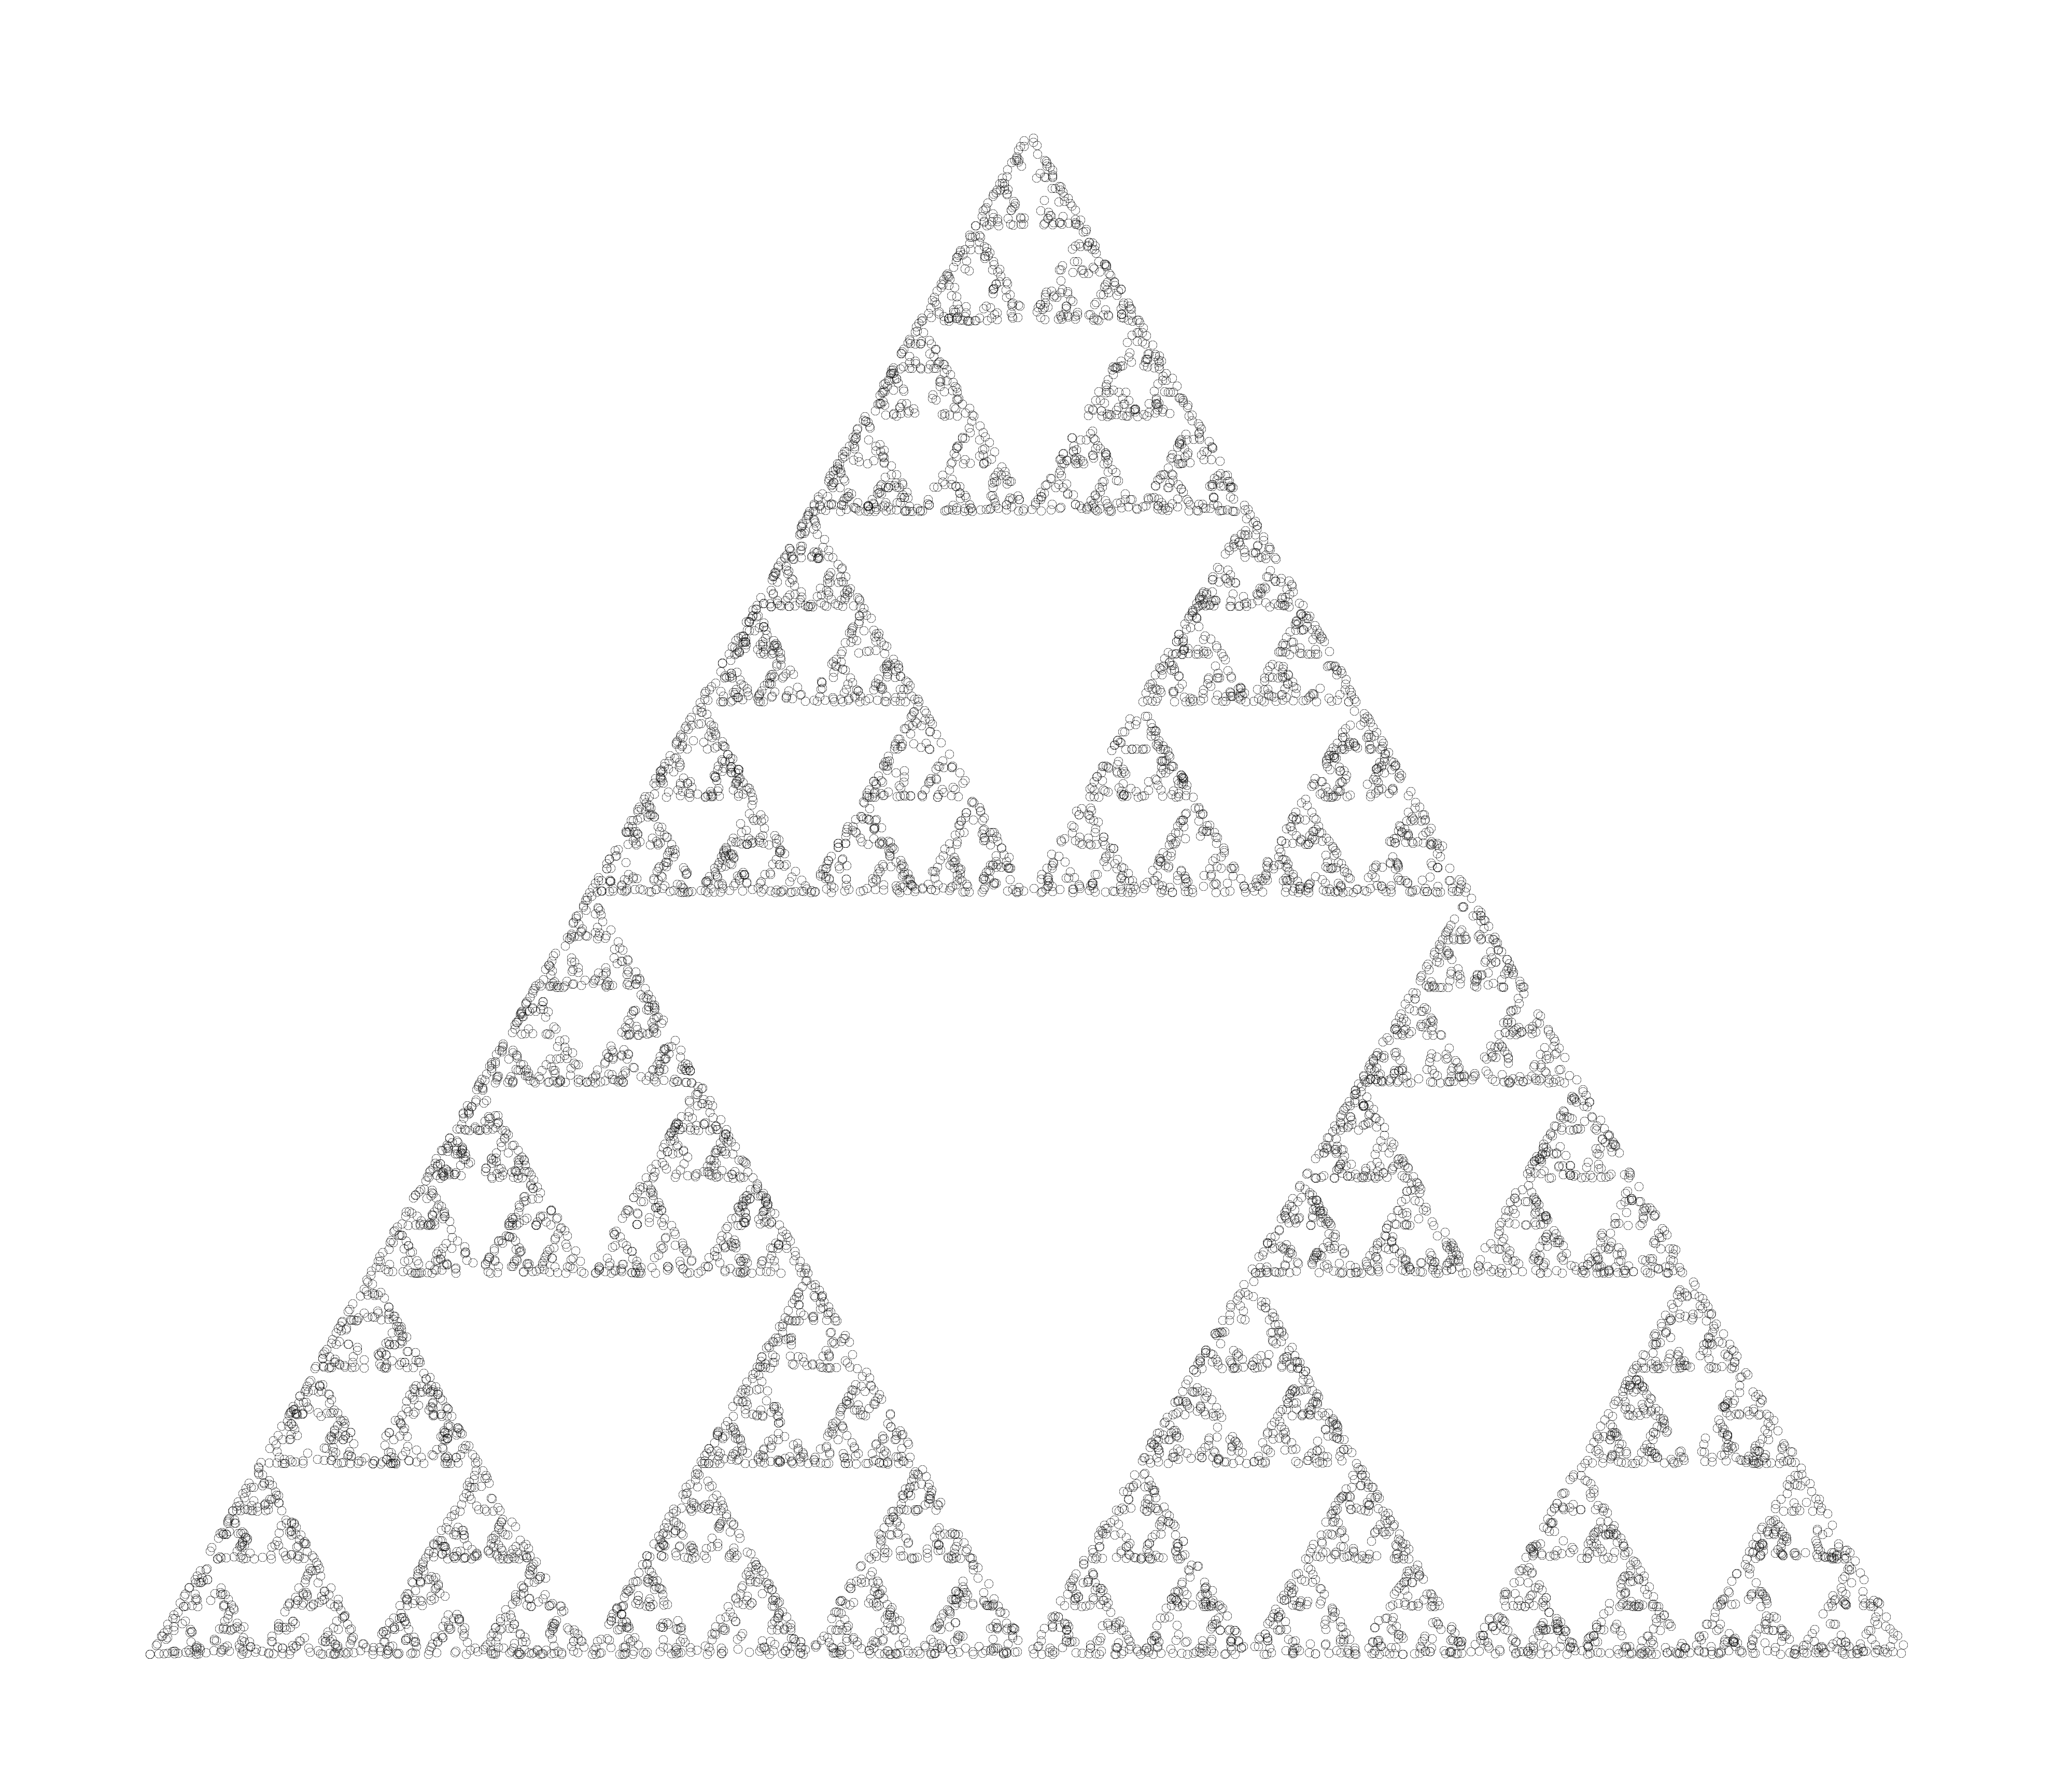
\includegraphics[width=.28\textwidth]{sierpinsky_triangle_2}%
    \hfill
    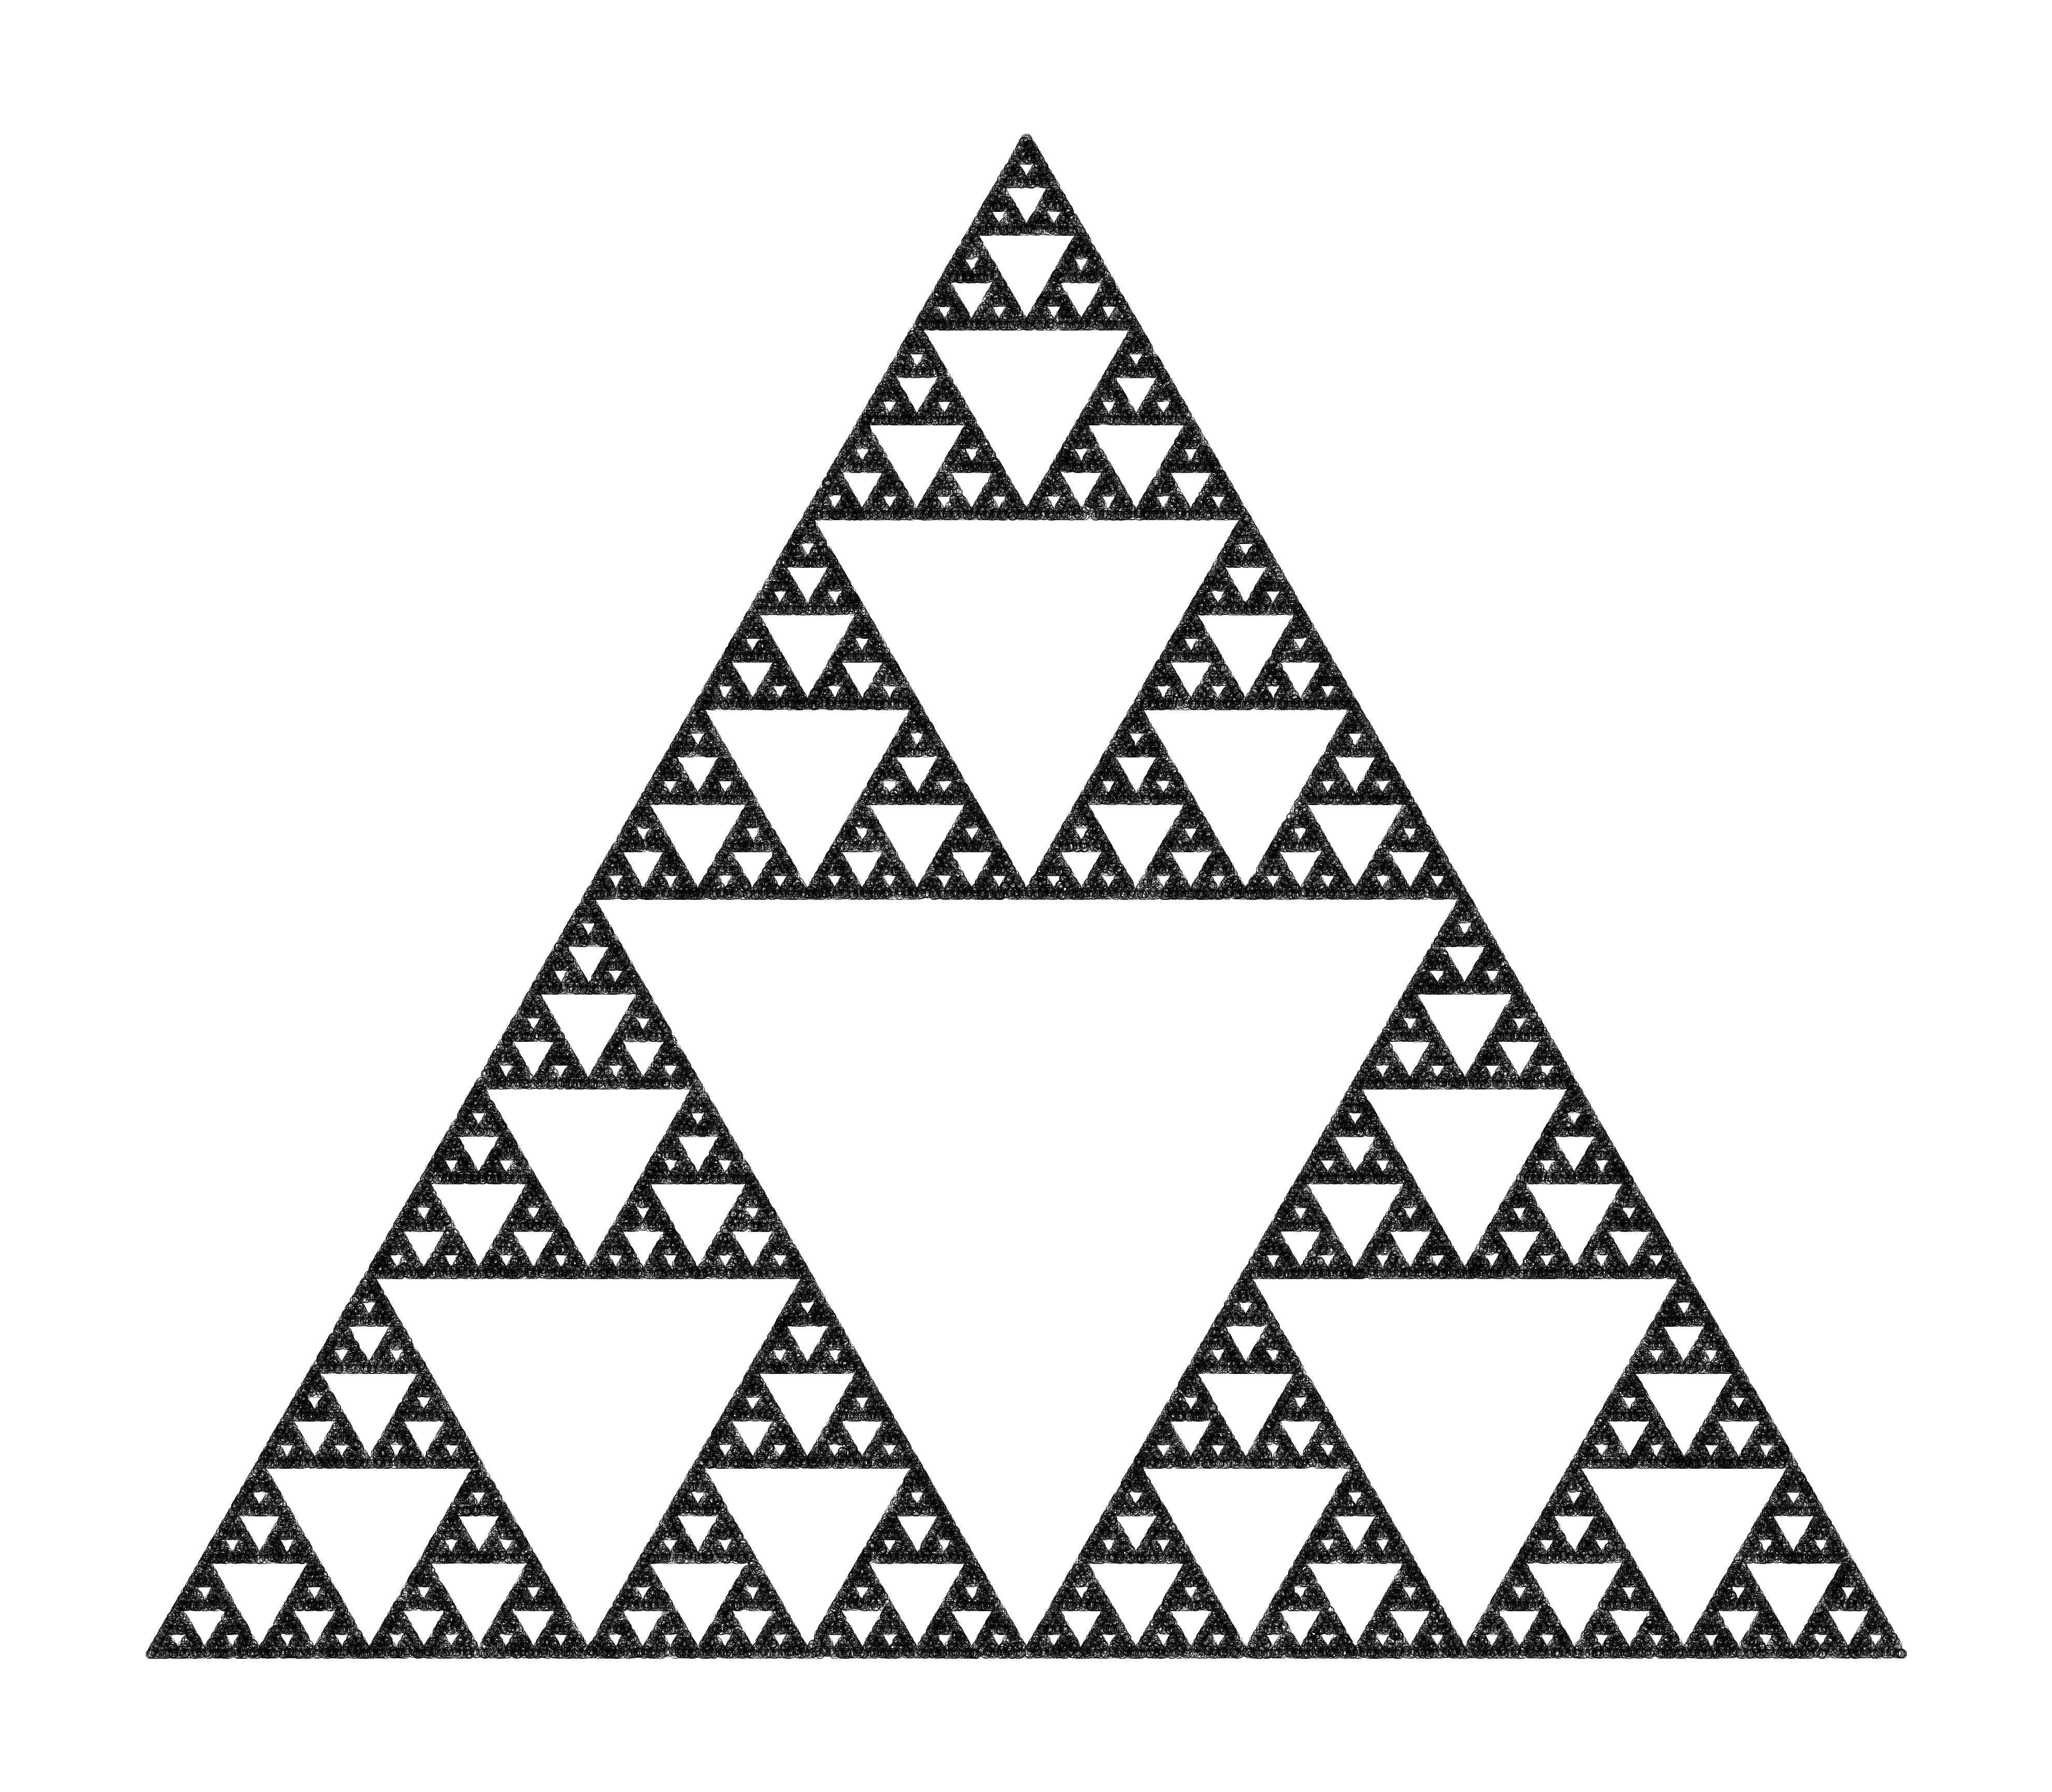
\includegraphics[width=.28\textwidth]{sierpinsky_triangle_3}

    \vfill
  \end{frame}

  \begin{frame}
    \vfill

    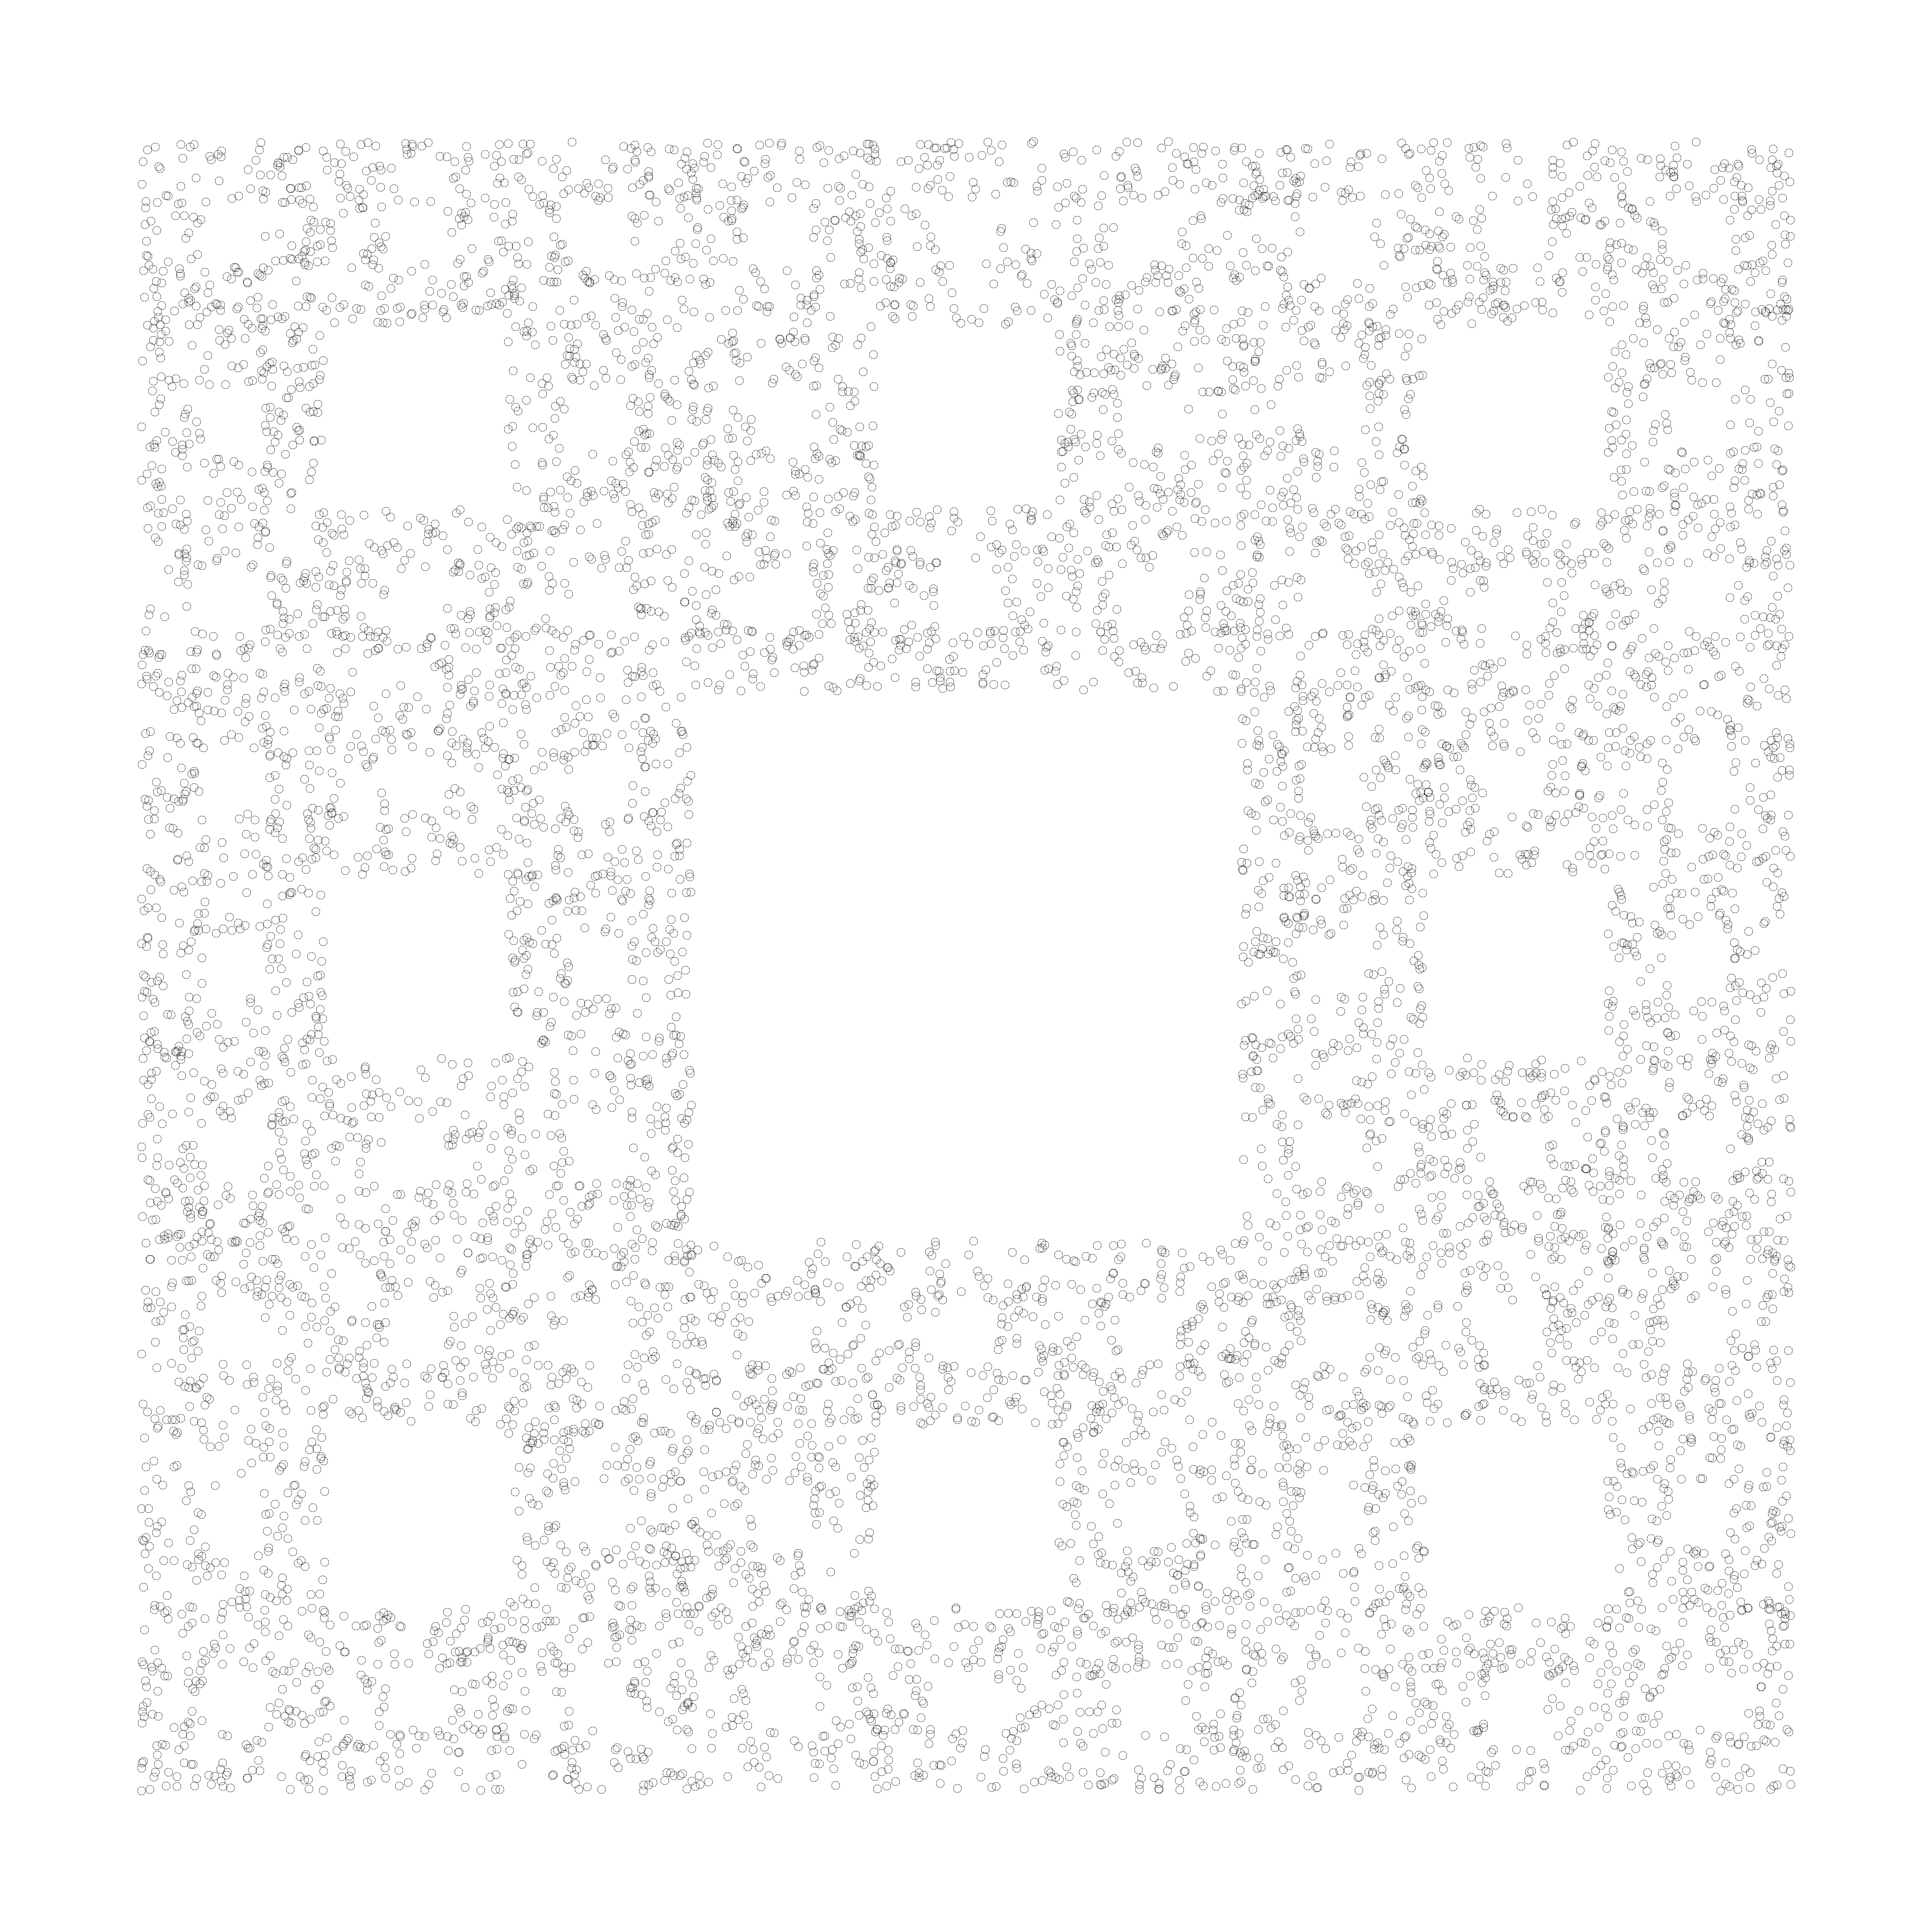
\includegraphics[width=.28\textwidth]{sierpinsky_carpet_1}%
    \hfill
    \includegraphics[width=.28\textwidth]{sierpinsky_carpet_2}%
    \hfill
    \includegraphics[width=.28\textwidth]{sierpinsky_carpet_3}

    \vfill
  \end{frame}
}


\begin{frame}
  \vfill
  \large

  \begin{minipage}{.48\textwidth}
    \[
    f_1(x, y)
    =
    \begin{bmatrix}
      0 & 0 \\ 0 & 0.16
    \end{bmatrix}
    \begin{bmatrix}
      x \\ y
    \end{bmatrix}
    \]
  \end{minipage}%
  \hfill
  \begin{minipage}{.48\textwidth}
    \[
    f_2(x, y)
    =
    \begin{bmatrix}
      0.85 & 0.04 \\ -0.04 & 0.85
    \end{bmatrix}
    \begin{bmatrix}
      x \\ y
    \end{bmatrix}
    +
    \begin{bmatrix}
      0 \\ 1.6
    \end{bmatrix}
    \]
  \end{minipage}

  \vfill

  \begin{minipage}{.48\textwidth}
    \[
    f_3(x, y)
    =
    \begin{bmatrix}
      0.2 & -0.26 \\ 0.23 & 0.22
    \end{bmatrix}
    \begin{bmatrix}
      x \\ y
    \end{bmatrix}
    +
    \begin{bmatrix}
      0 \\ 1.6
    \end{bmatrix}
    \]
  \end{minipage}%
  \hfill
  \begin{minipage}{.48\textwidth}
    \[
    f_4(x, y)
    =
    \begin{bmatrix}
      -0.15 & 0.28 \\ -0.26 & 0.24
    \end{bmatrix}
    \begin{bmatrix}
      x \\ y
    \end{bmatrix}
    +
    \begin{bmatrix}
      0 \\ 0.44
    \end{bmatrix}
    \]
  \end{minipage}


  \vfill
\end{frame}

{
  \setbeamercolor{background canvas}{bg=white}
  \setbeamercolor{background canvas}{bg=white}
  \setbeamercolor{normal text}{fg=black}

  \usebeamercolor[fg]{normal text}

  \setbeamercolor{frametitle}{fg=black}
  \setbeamercolor{framesubtitle}{fg=black}
  \setbeamercolor{itemize item}{fg=black}

  \begin{frame}[fragile]{}{}
    \vfill
    \centering

    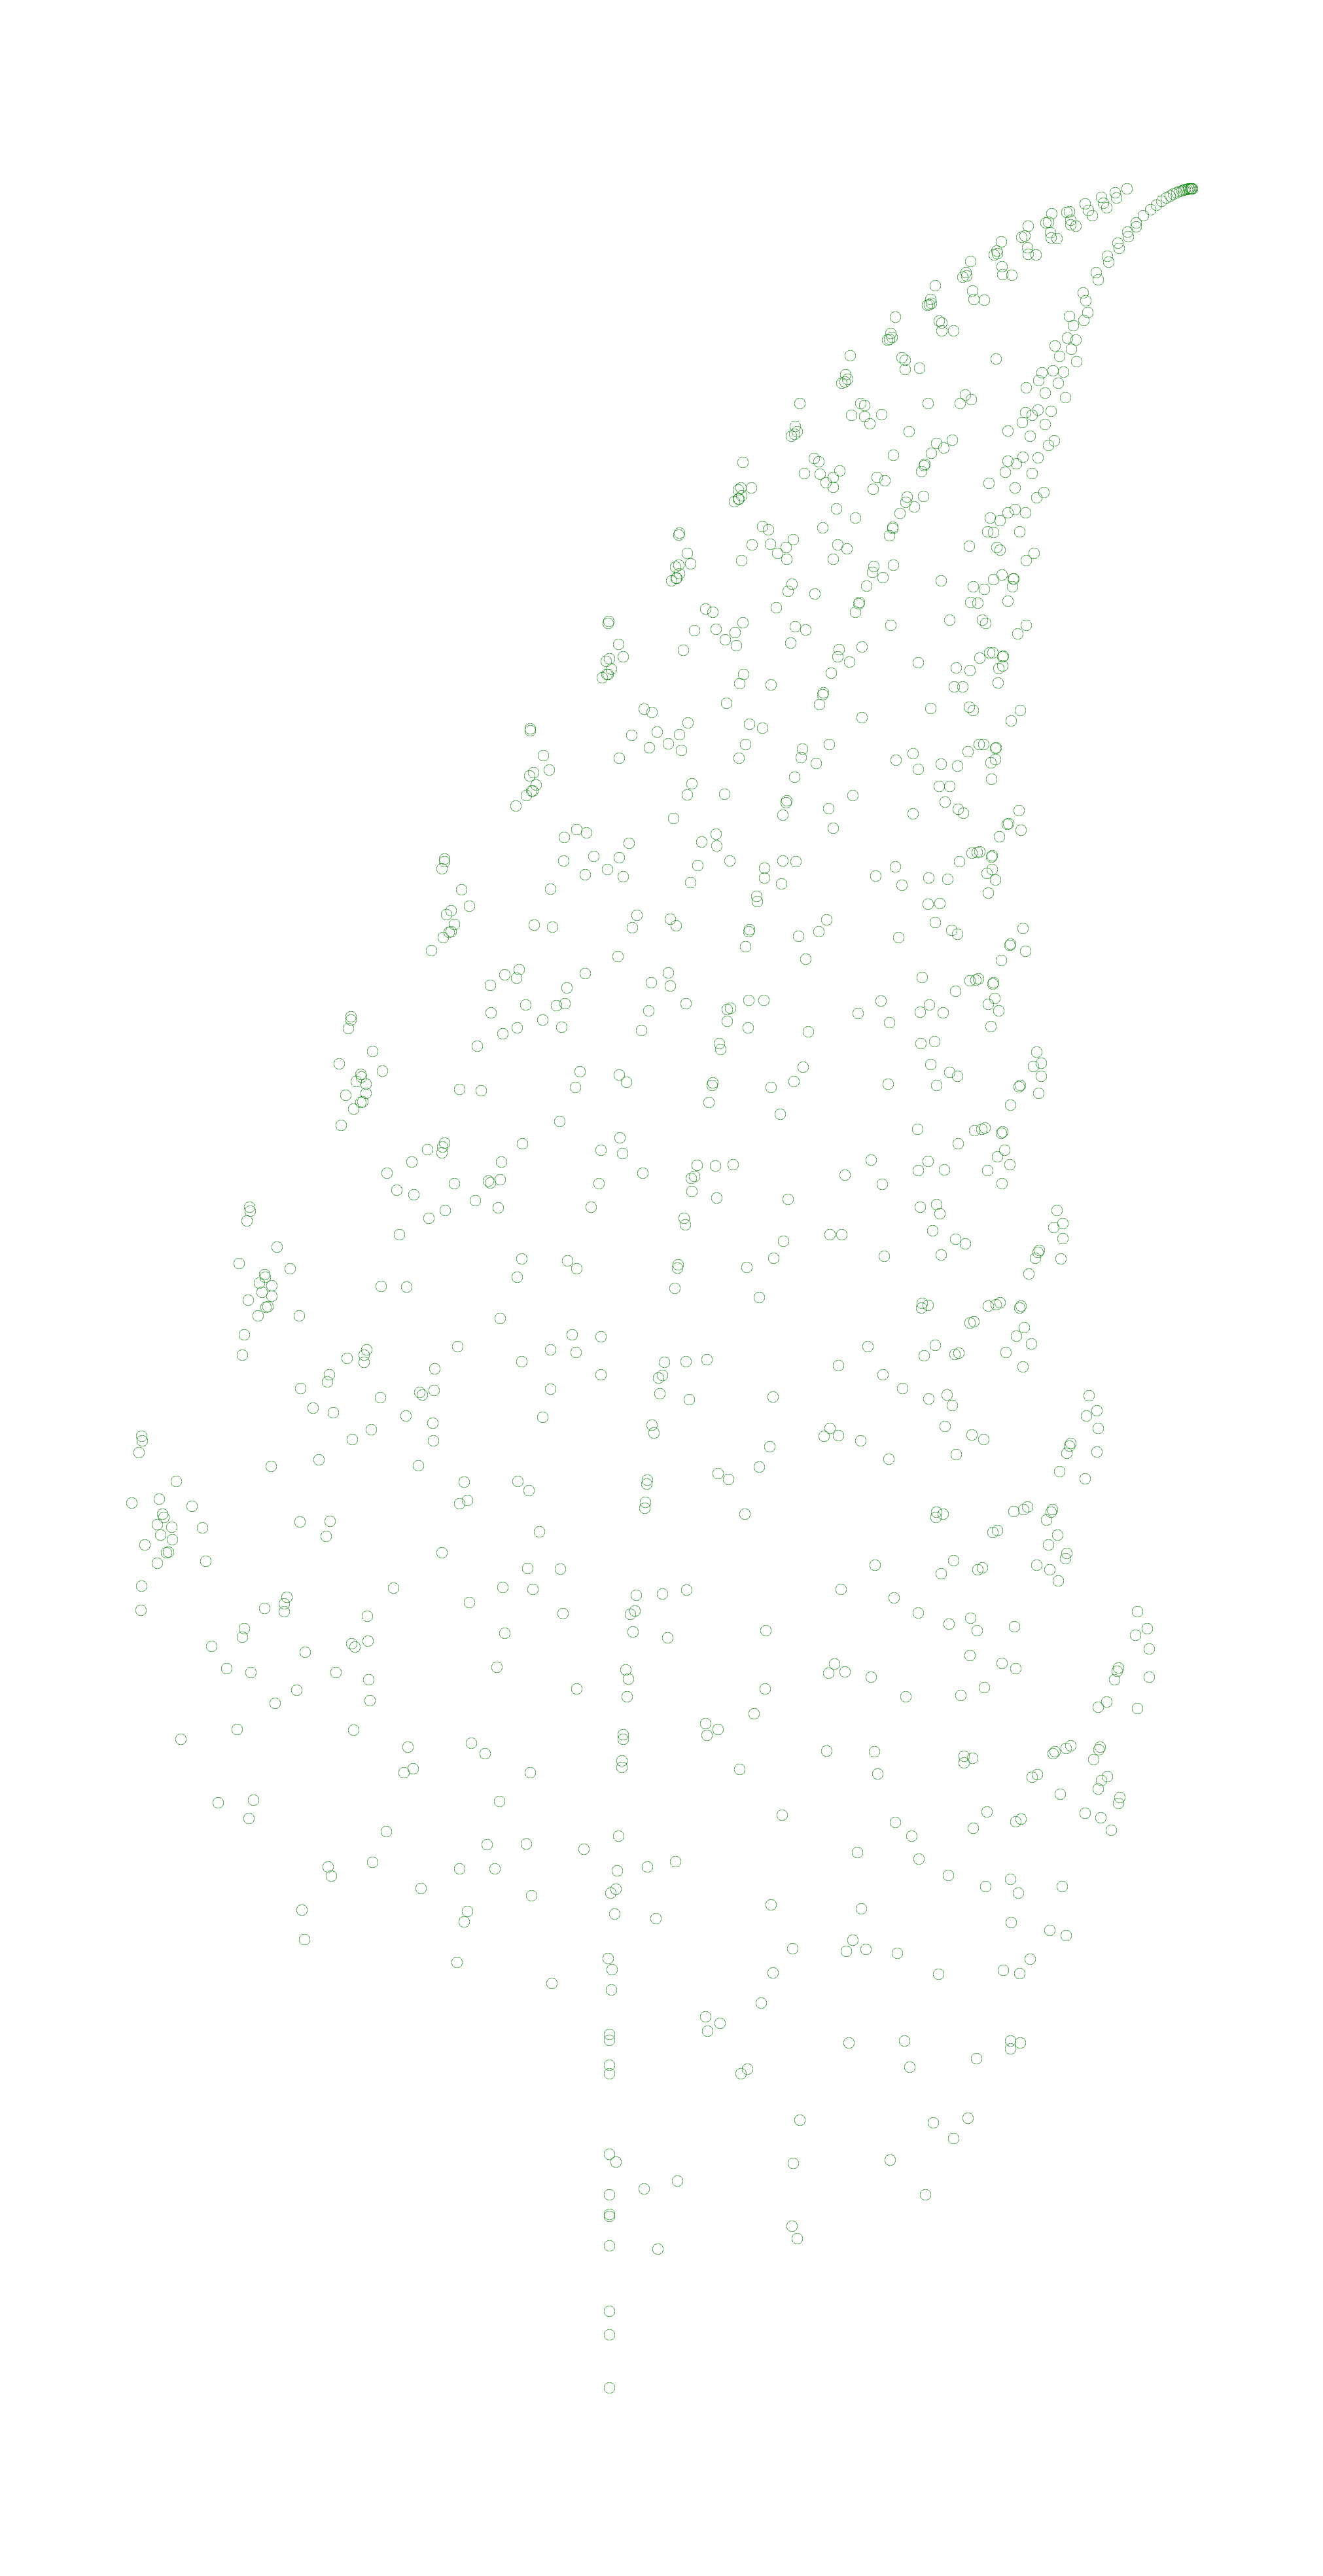
\includegraphics[height=.75\textheight]{barnsley_fern_1}%
    \hfill
    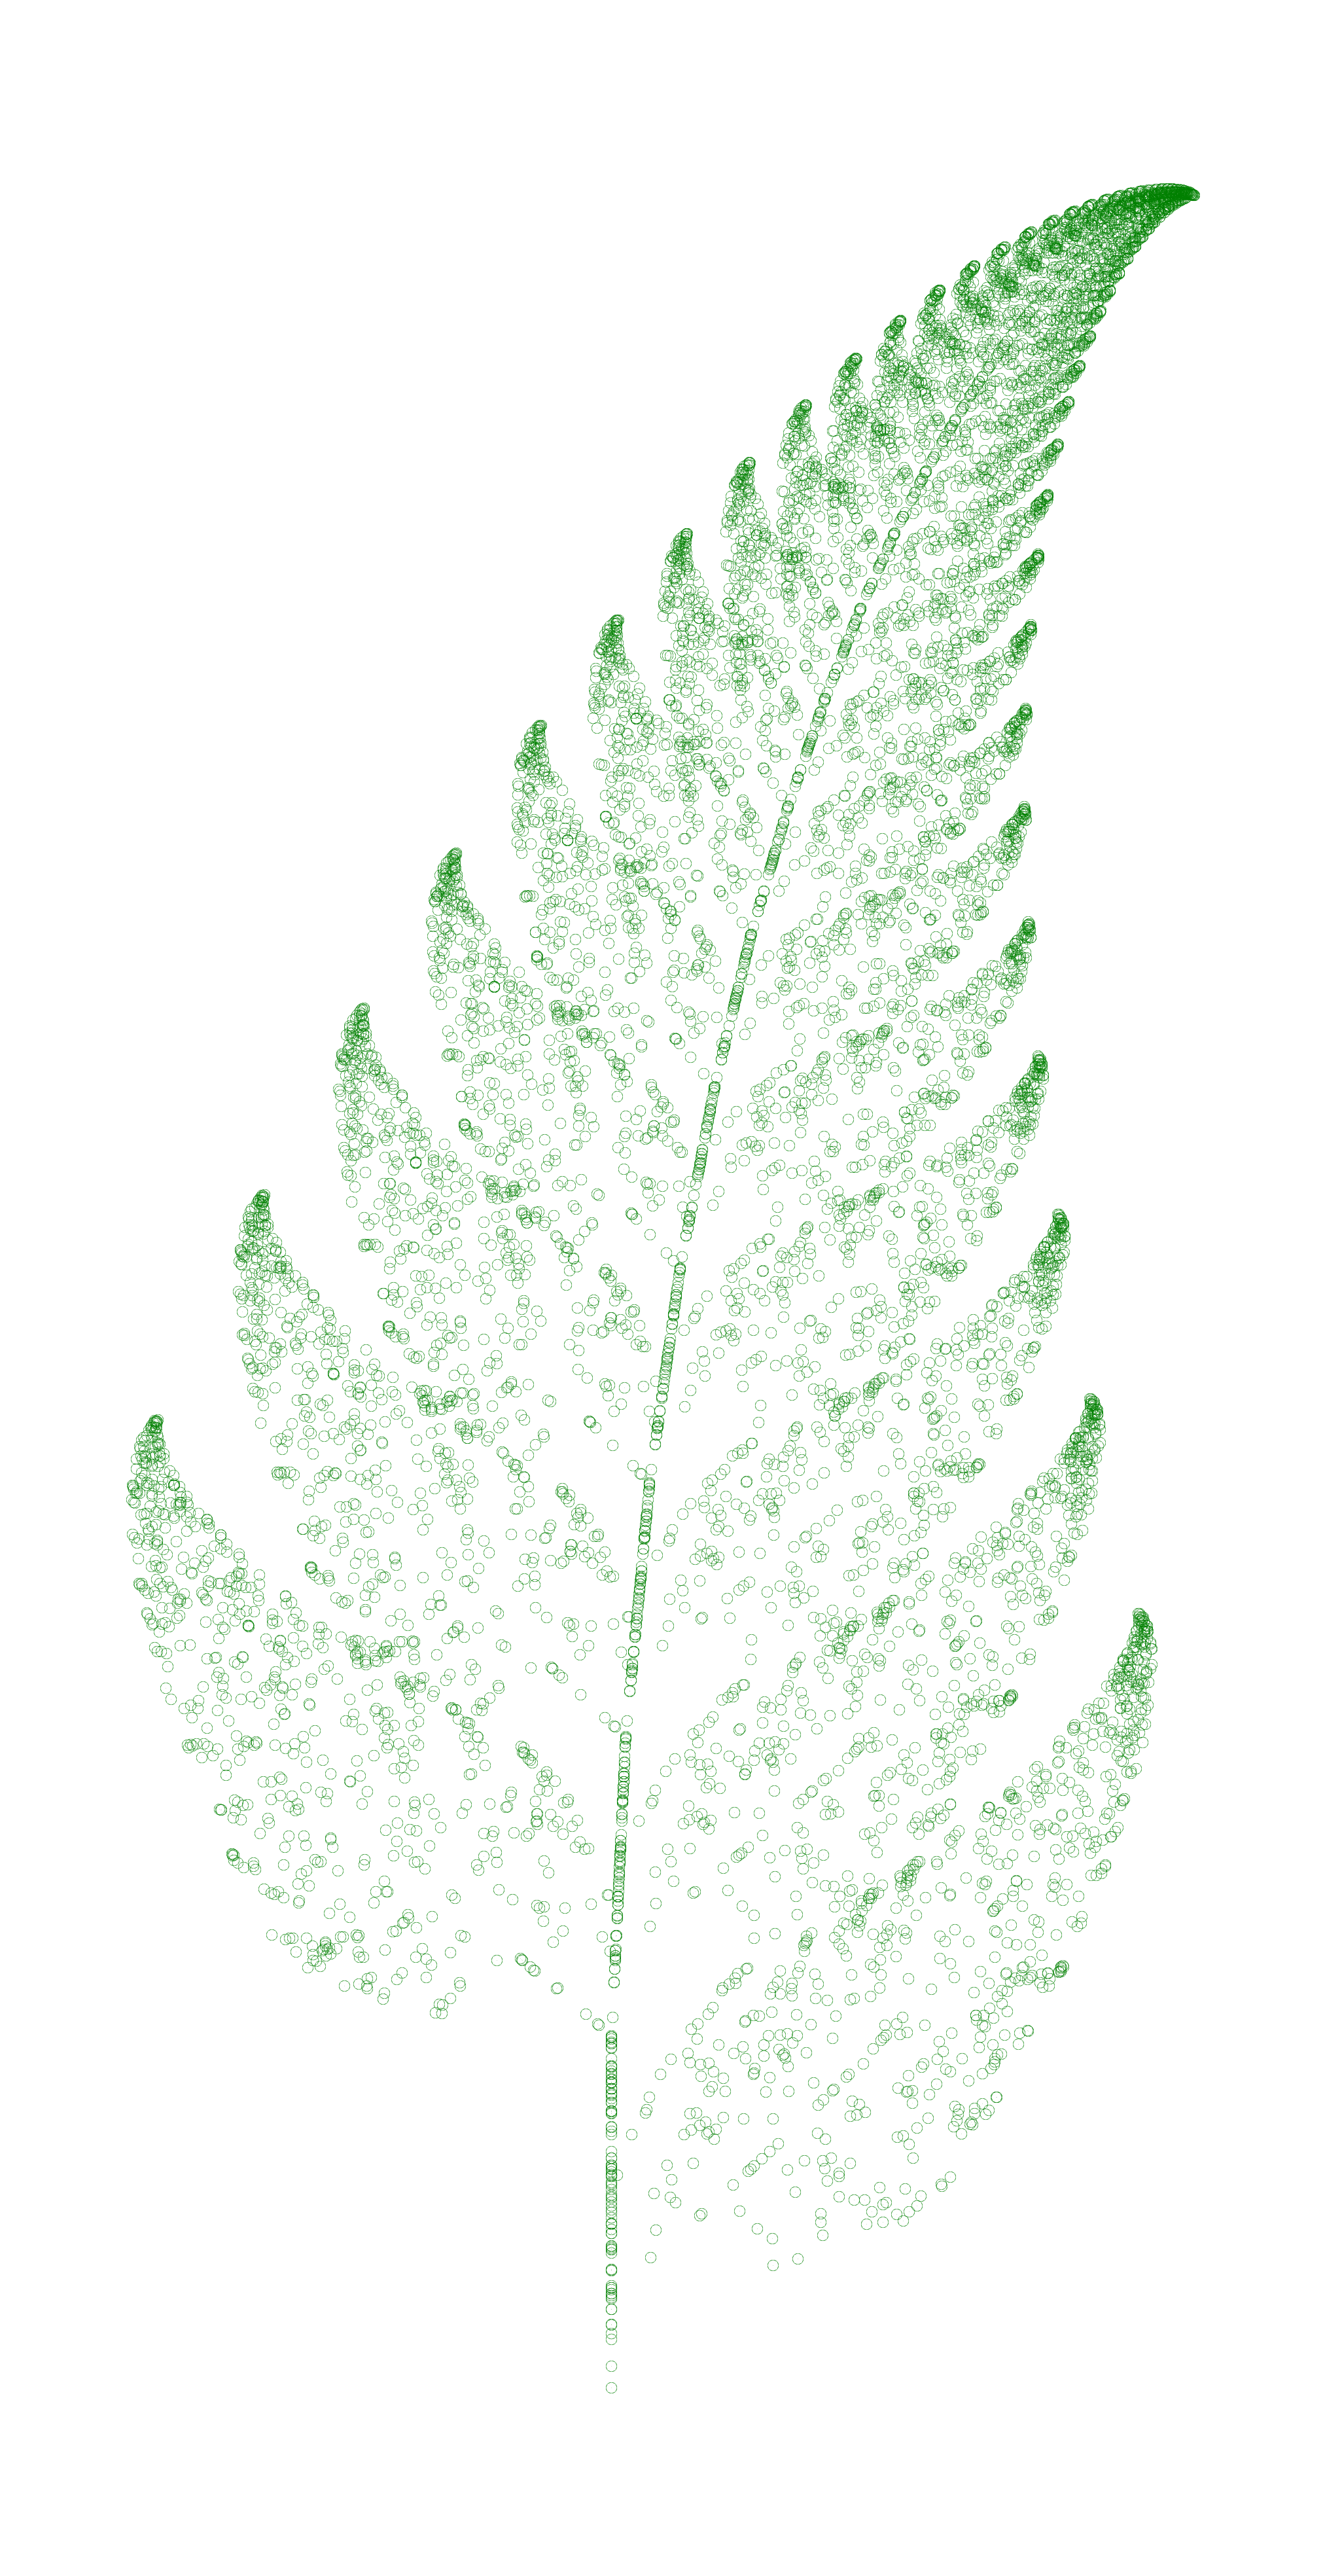
\includegraphics[height=.75\textheight]{barnsley_fern_2}%
    \hfill
    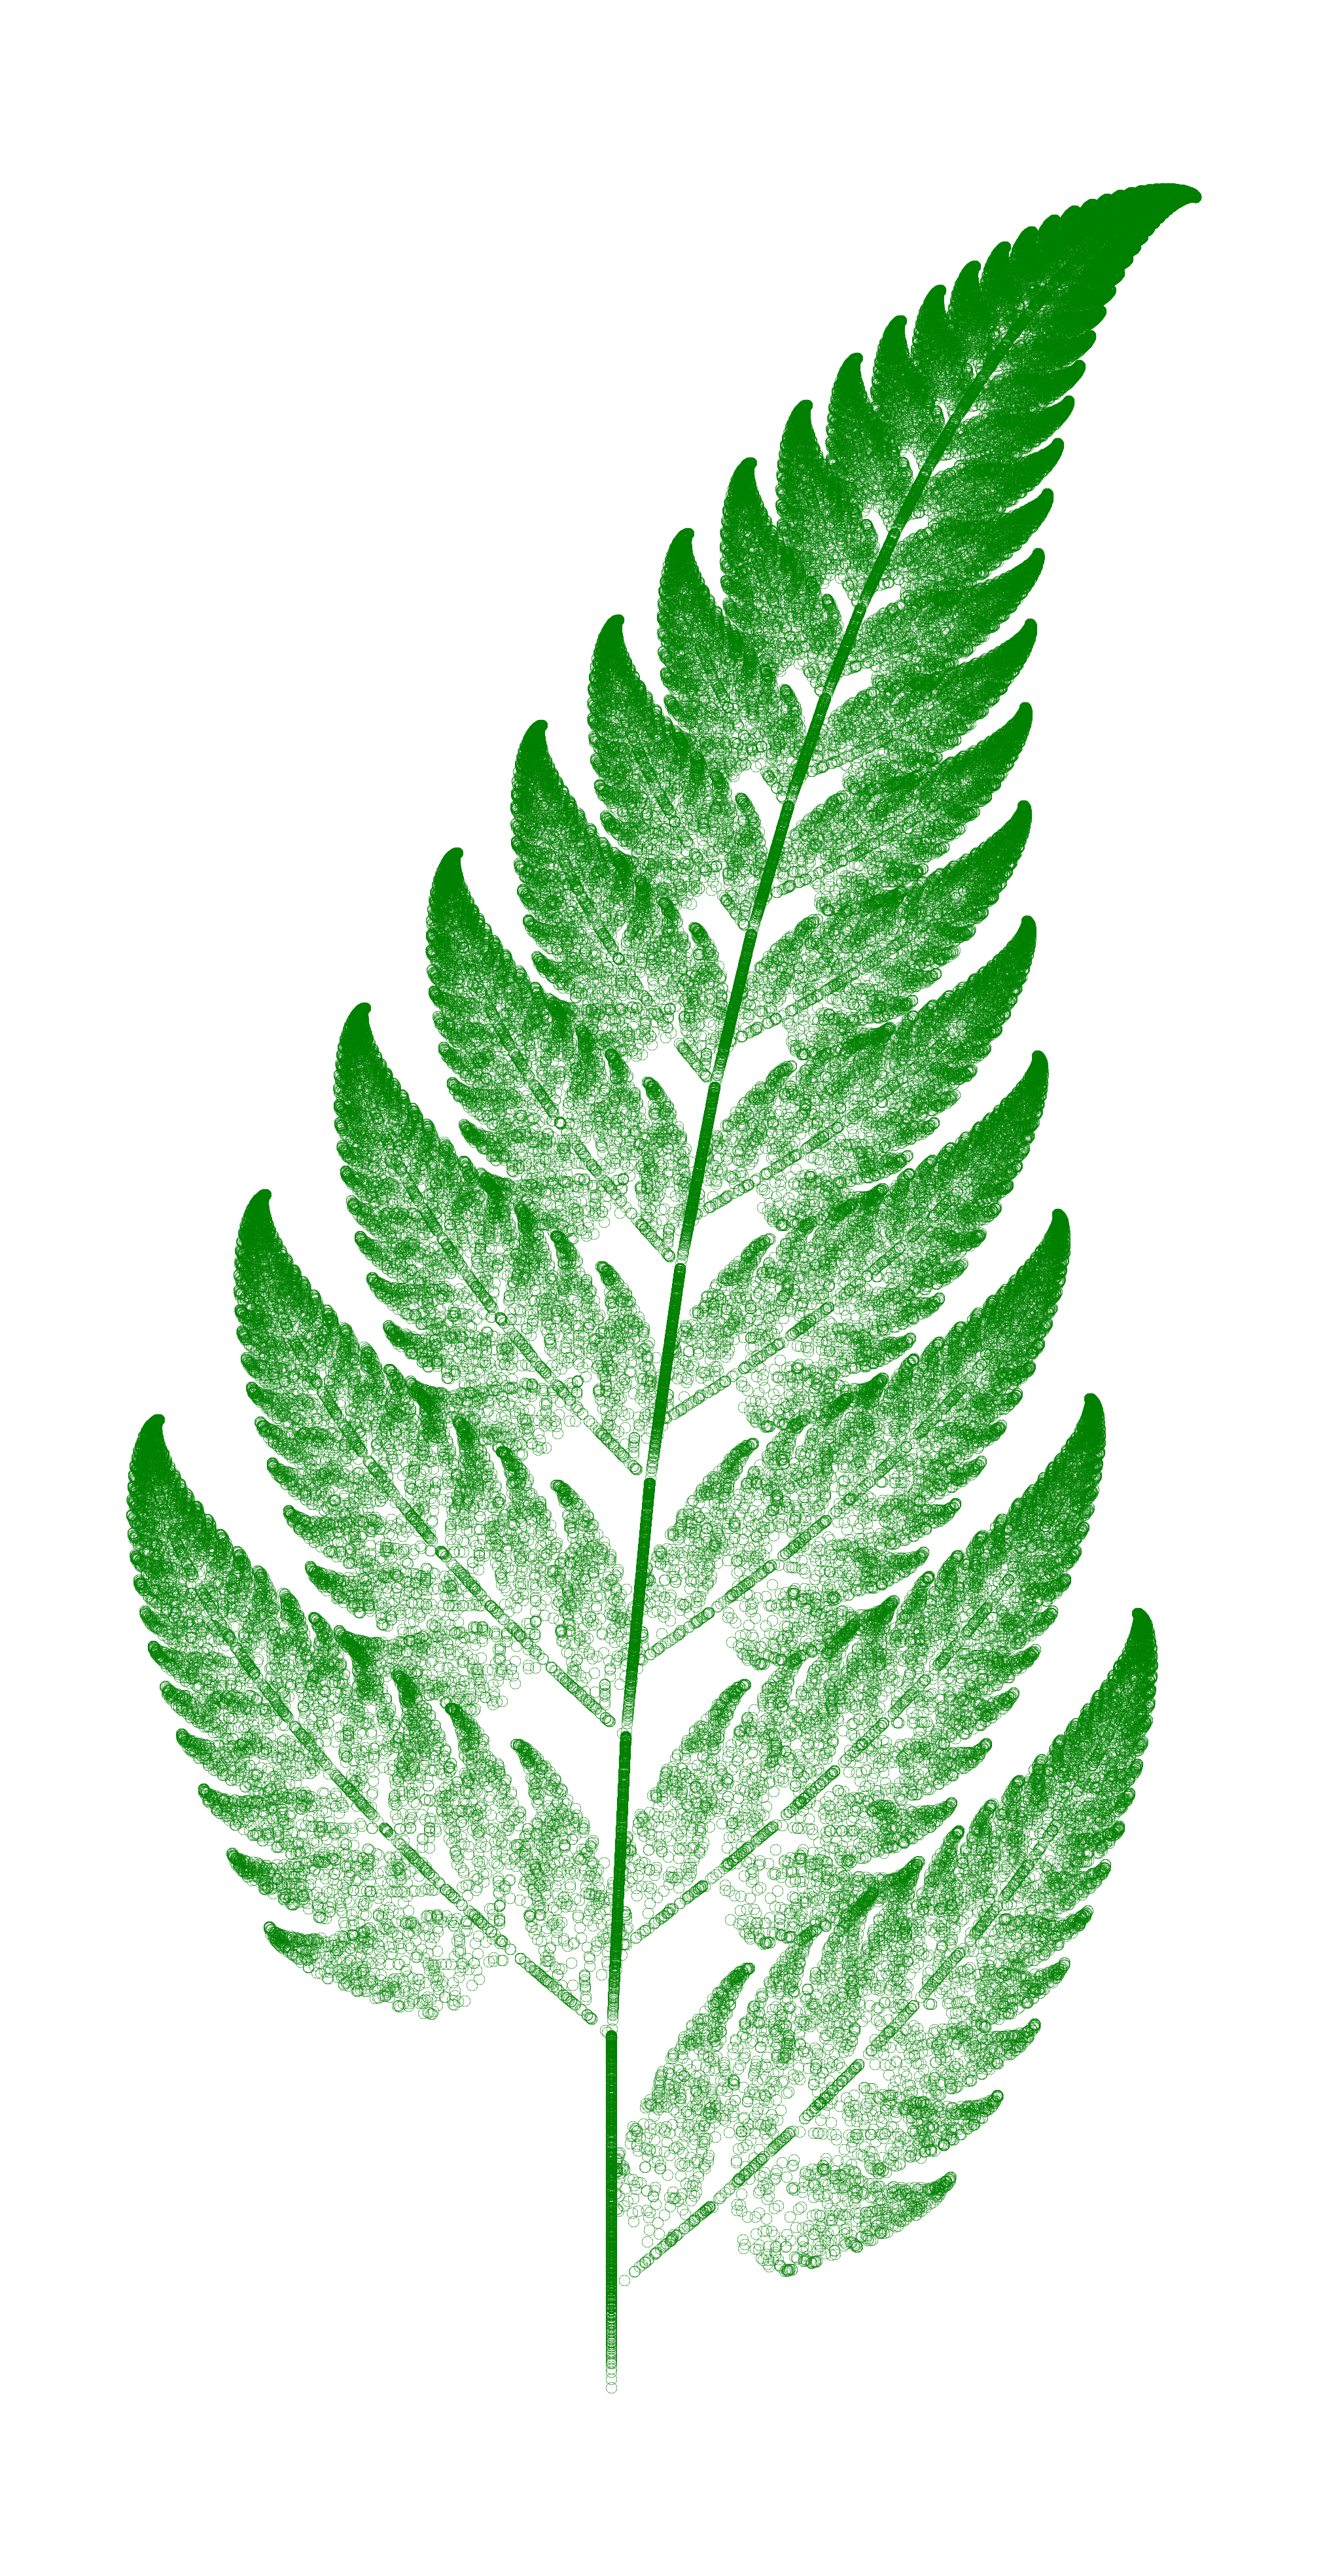
\includegraphics[height=.75\textheight]{barnsley_fern_3}

    \vfill
  \end{frame}

}

\begin{frame}
  \vfill
  \large

  \[
  \bm{f}_i(x, y)
  =
  \begin{bmatrix}
    r \cos(\theta) & -s \sin(\varphi) \\
    r \sin(\theta) & s \cos(\varphi)
  \end{bmatrix}
  \begin{bmatrix}
    x \\ y
  \end{bmatrix}
  +
  \begin{bmatrix}
    b_1 \\ b_2
  \end{bmatrix}
  \]

  \vfill
\end{frame}

{
  \setbeamercolor{background canvas}{bg=white}
  \setbeamercolor{background canvas}{bg=white}
  \setbeamercolor{normal text}{fg=black}

  \usebeamercolor[fg]{normal text}

  \setbeamercolor{frametitle}{fg=black}
  \setbeamercolor{framesubtitle}{fg=black}
  \setbeamercolor{itemize item}{fg=black}

  \begin{frame}[fragile]{}{}
    \vfill
    \centering

    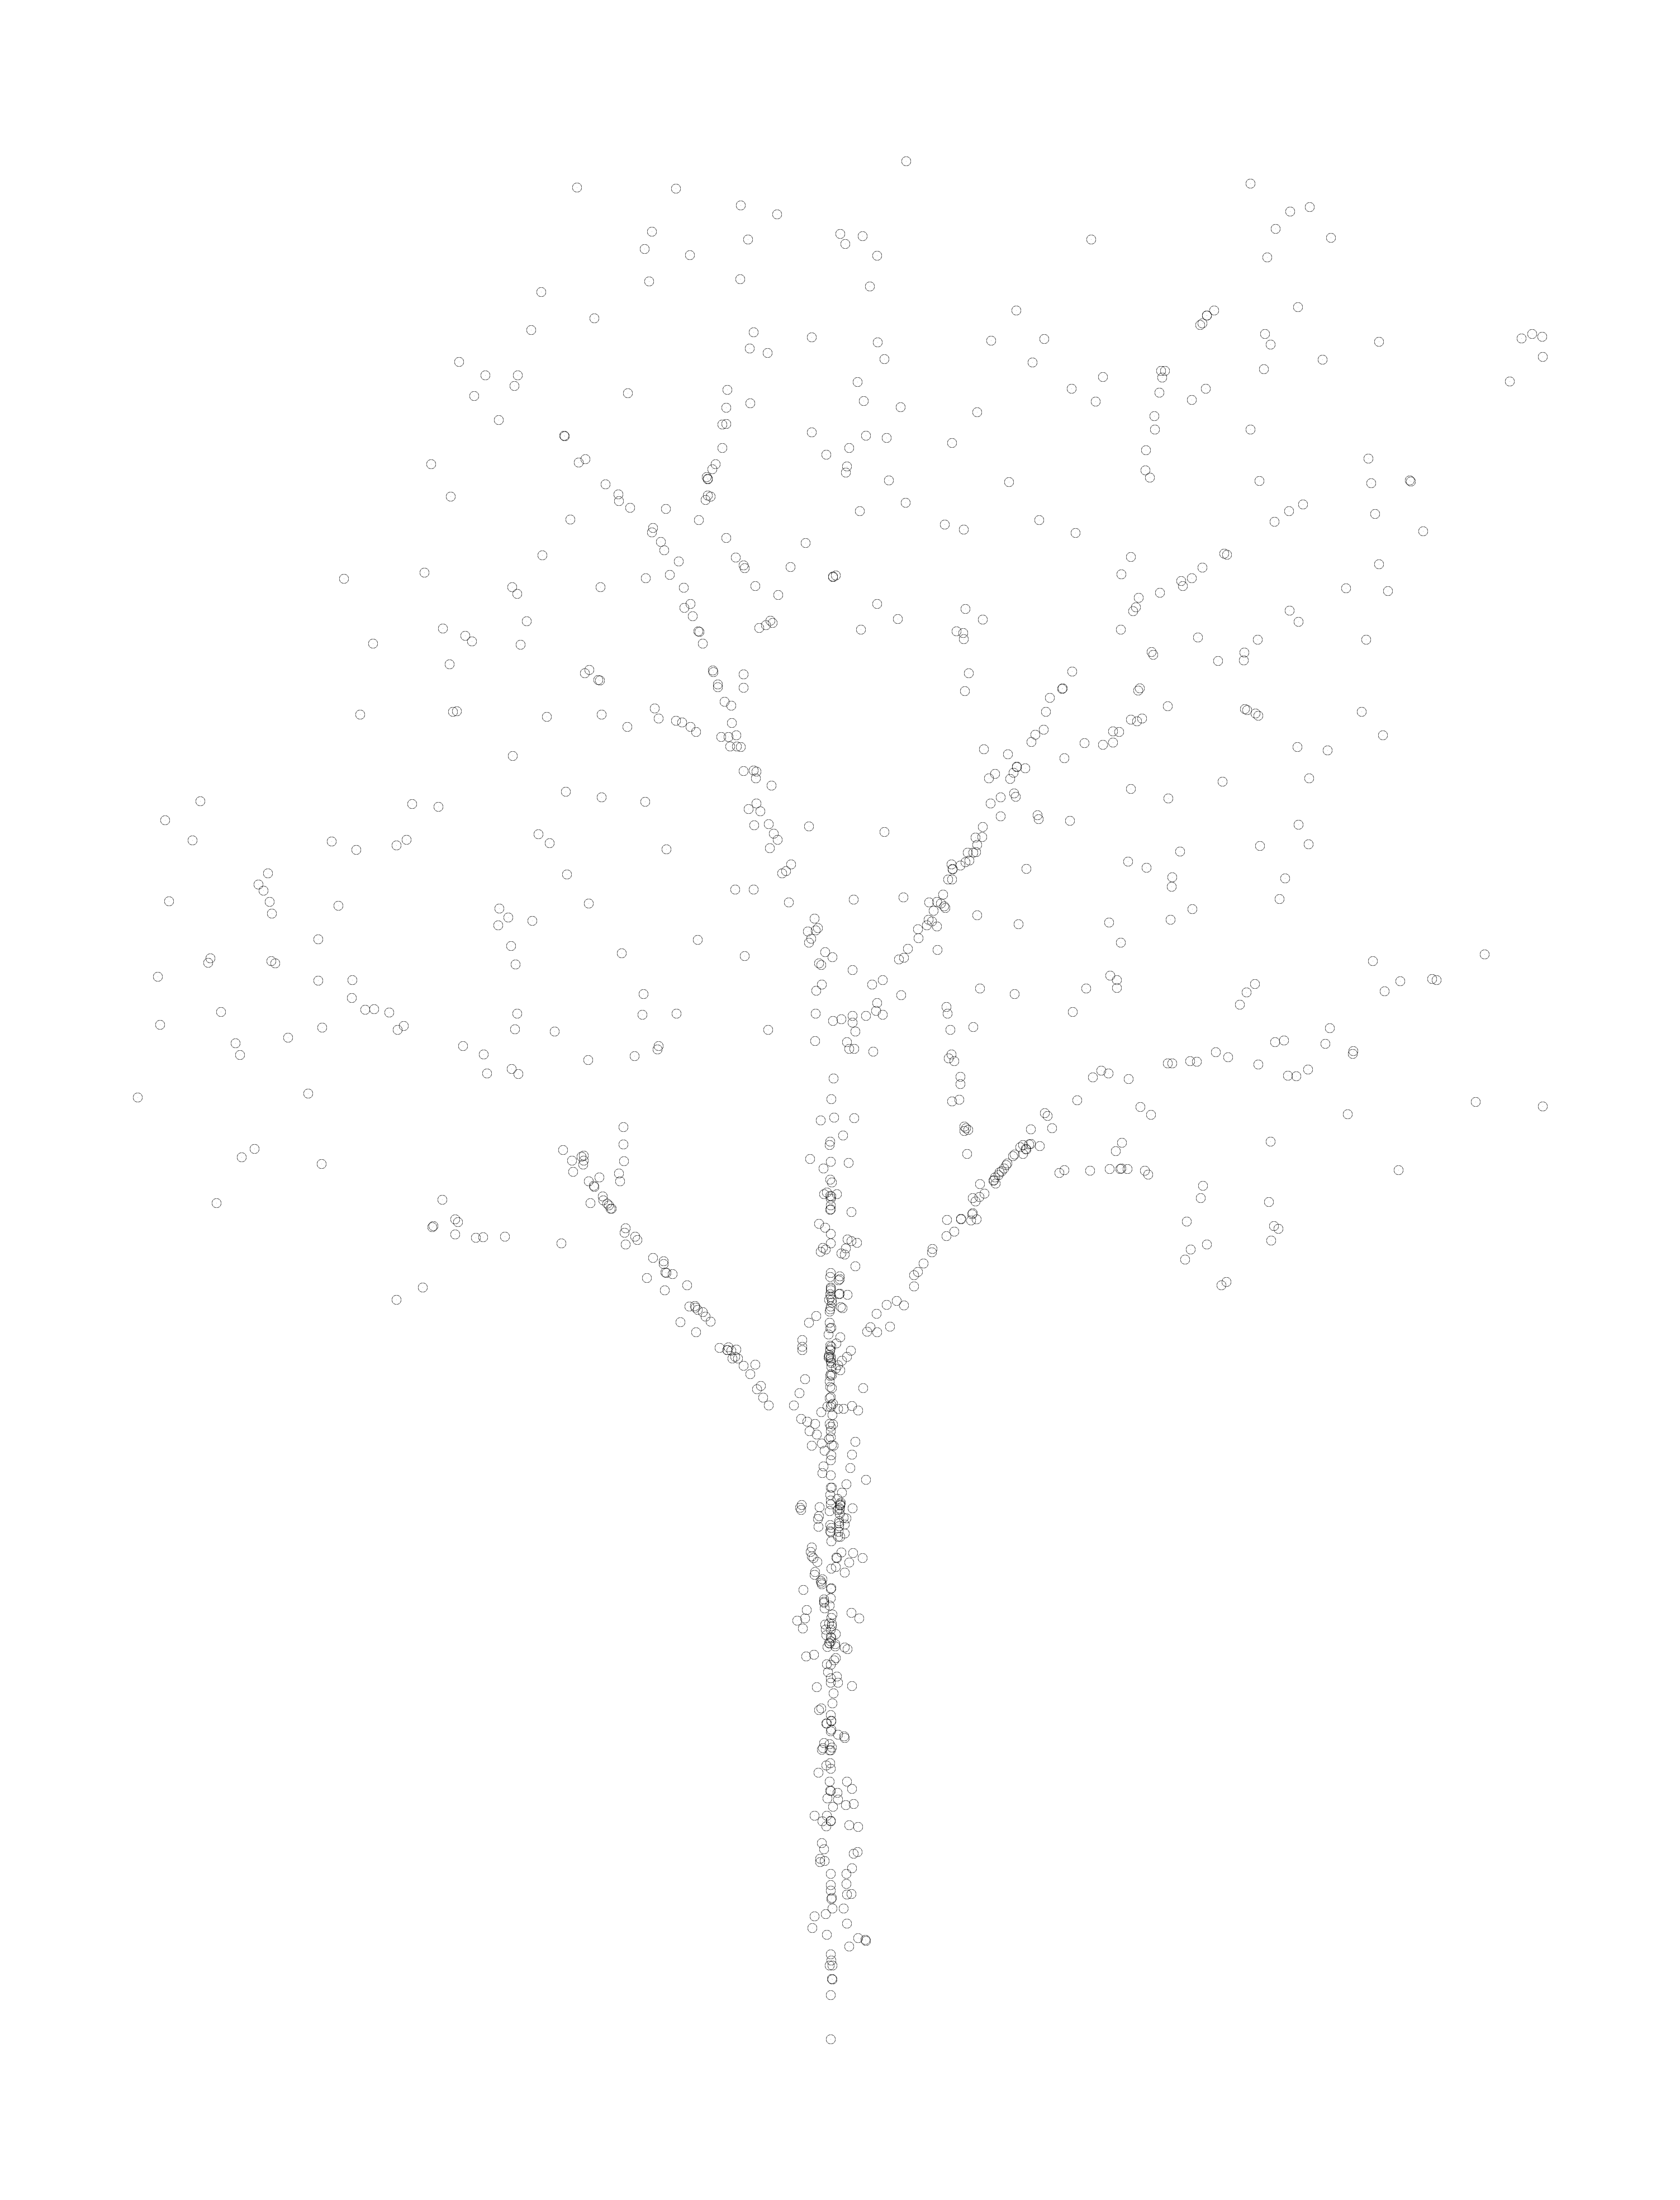
\includegraphics[width=.28\textwidth]{fractal_tree_1}%
    \hfill
    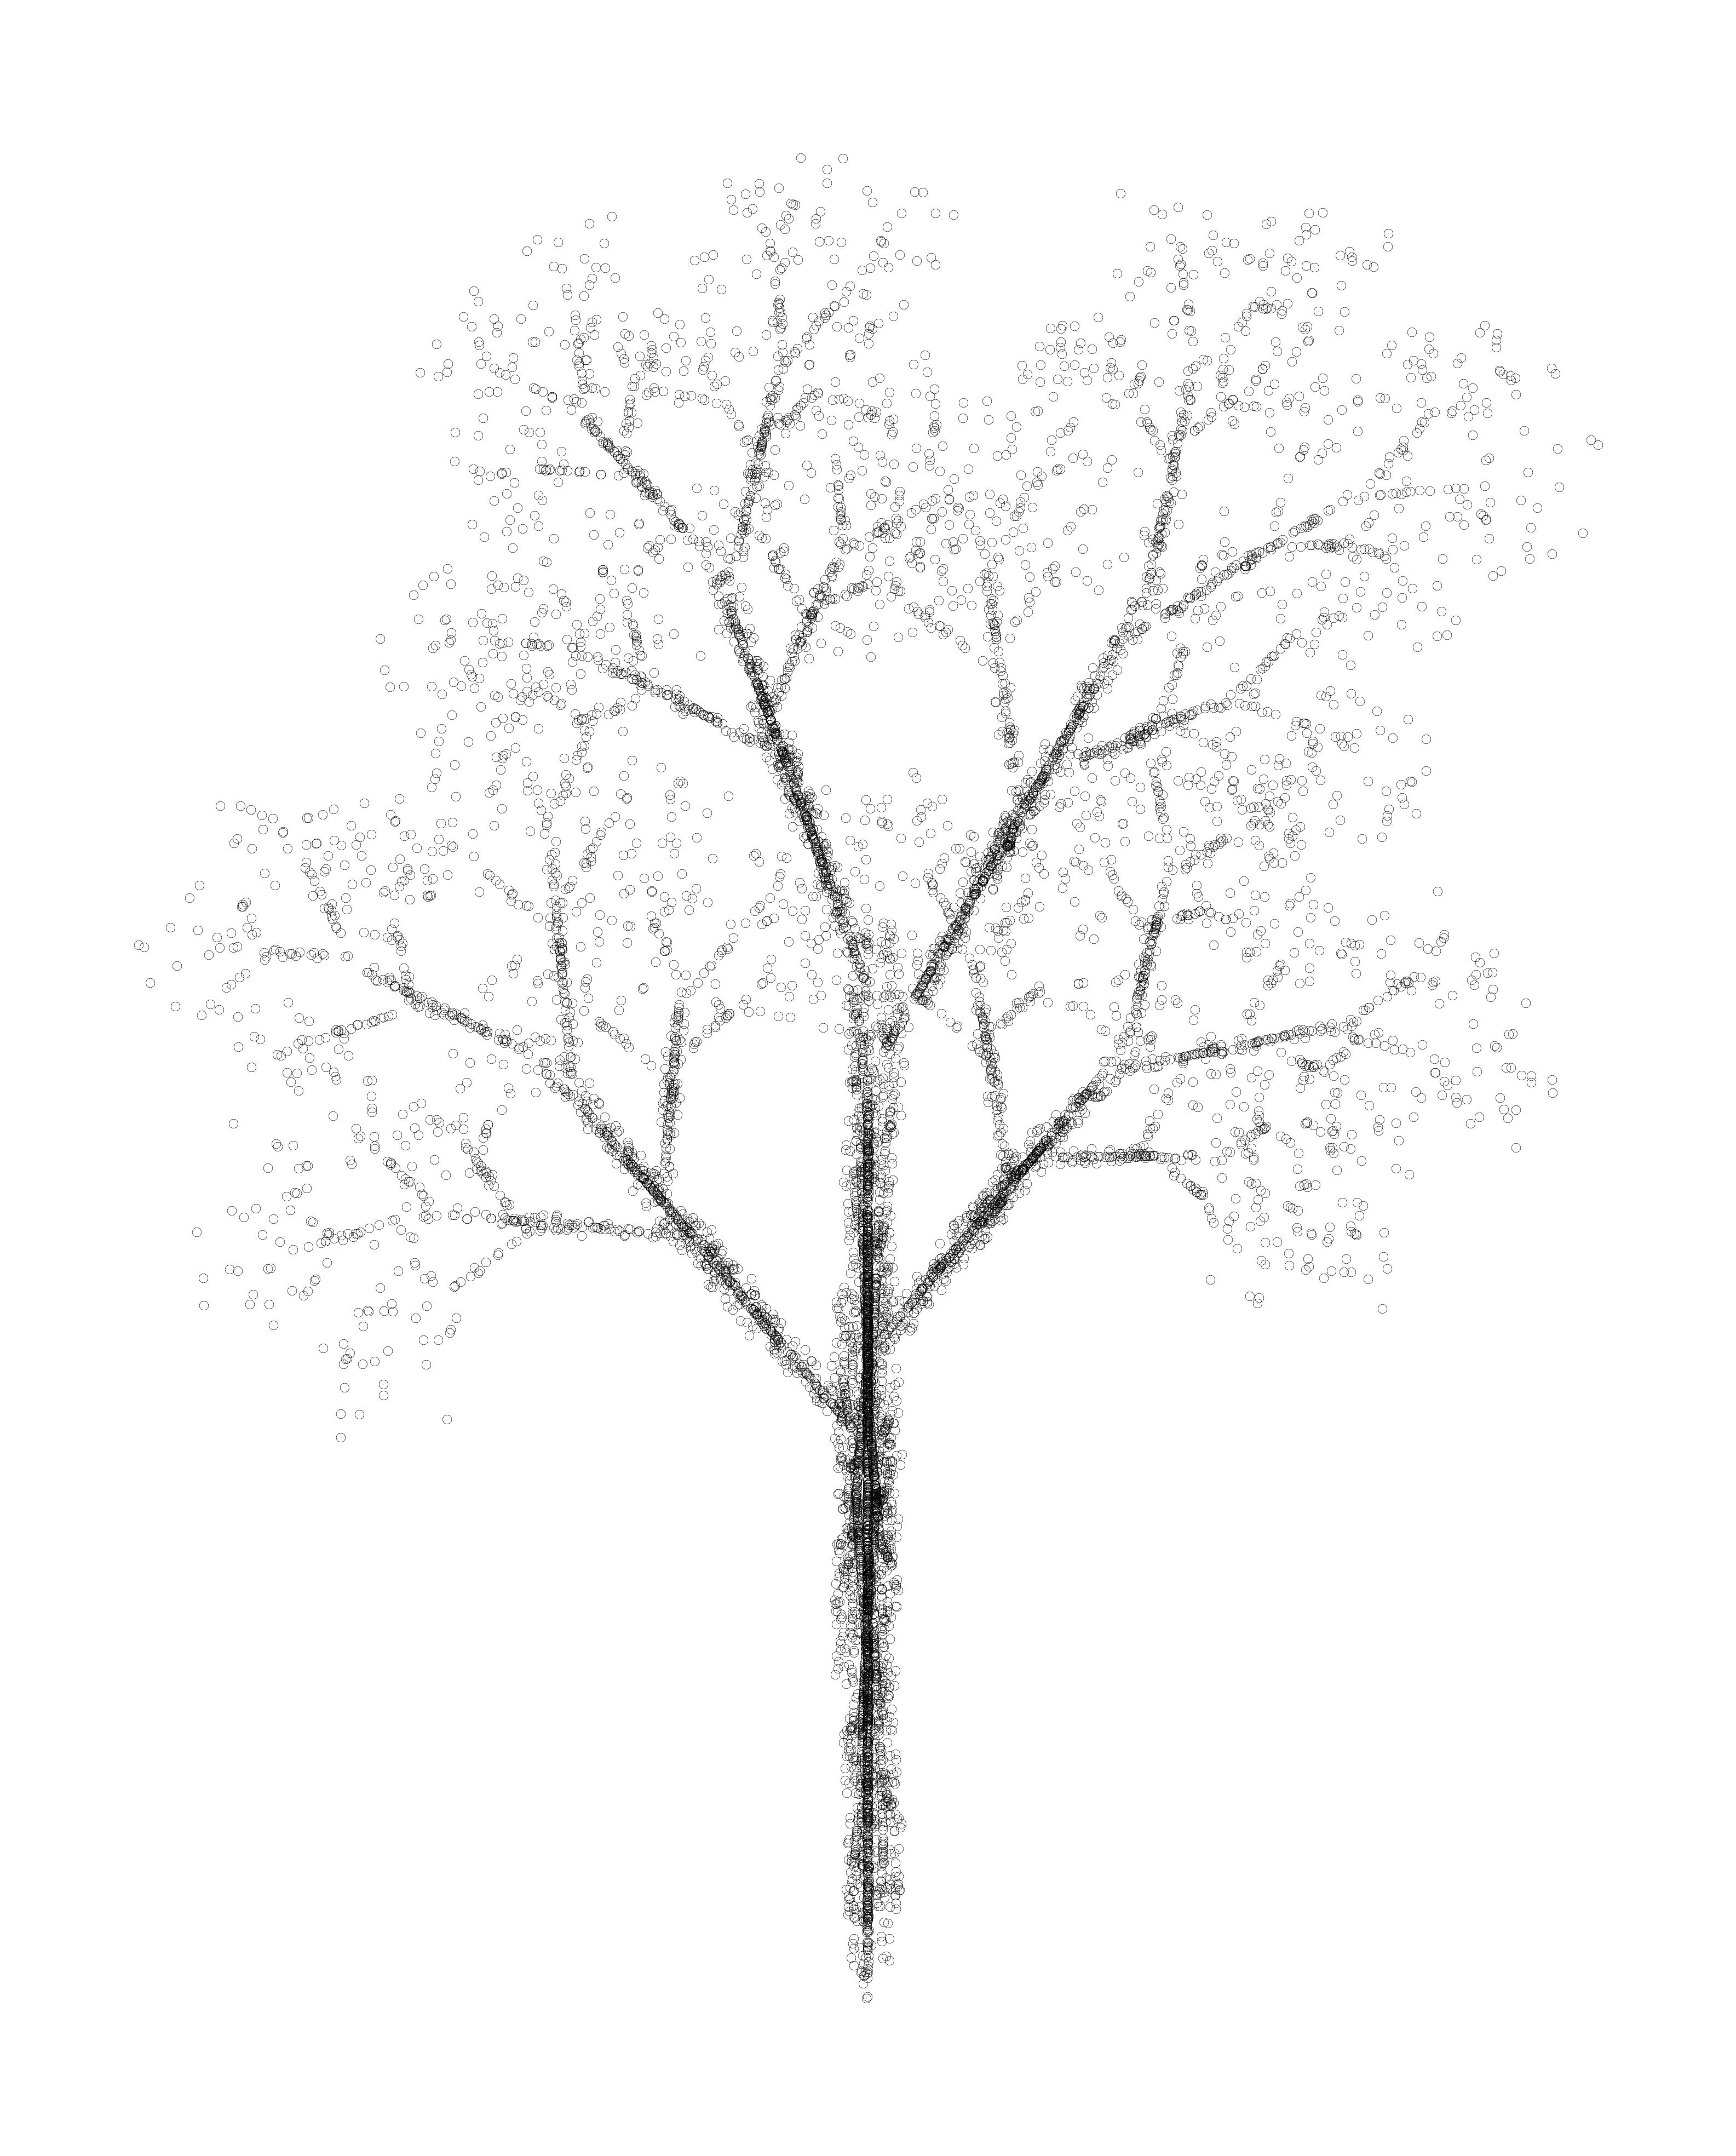
\includegraphics[width=.28\textwidth]{fractal_tree_2}%
    \hfill
    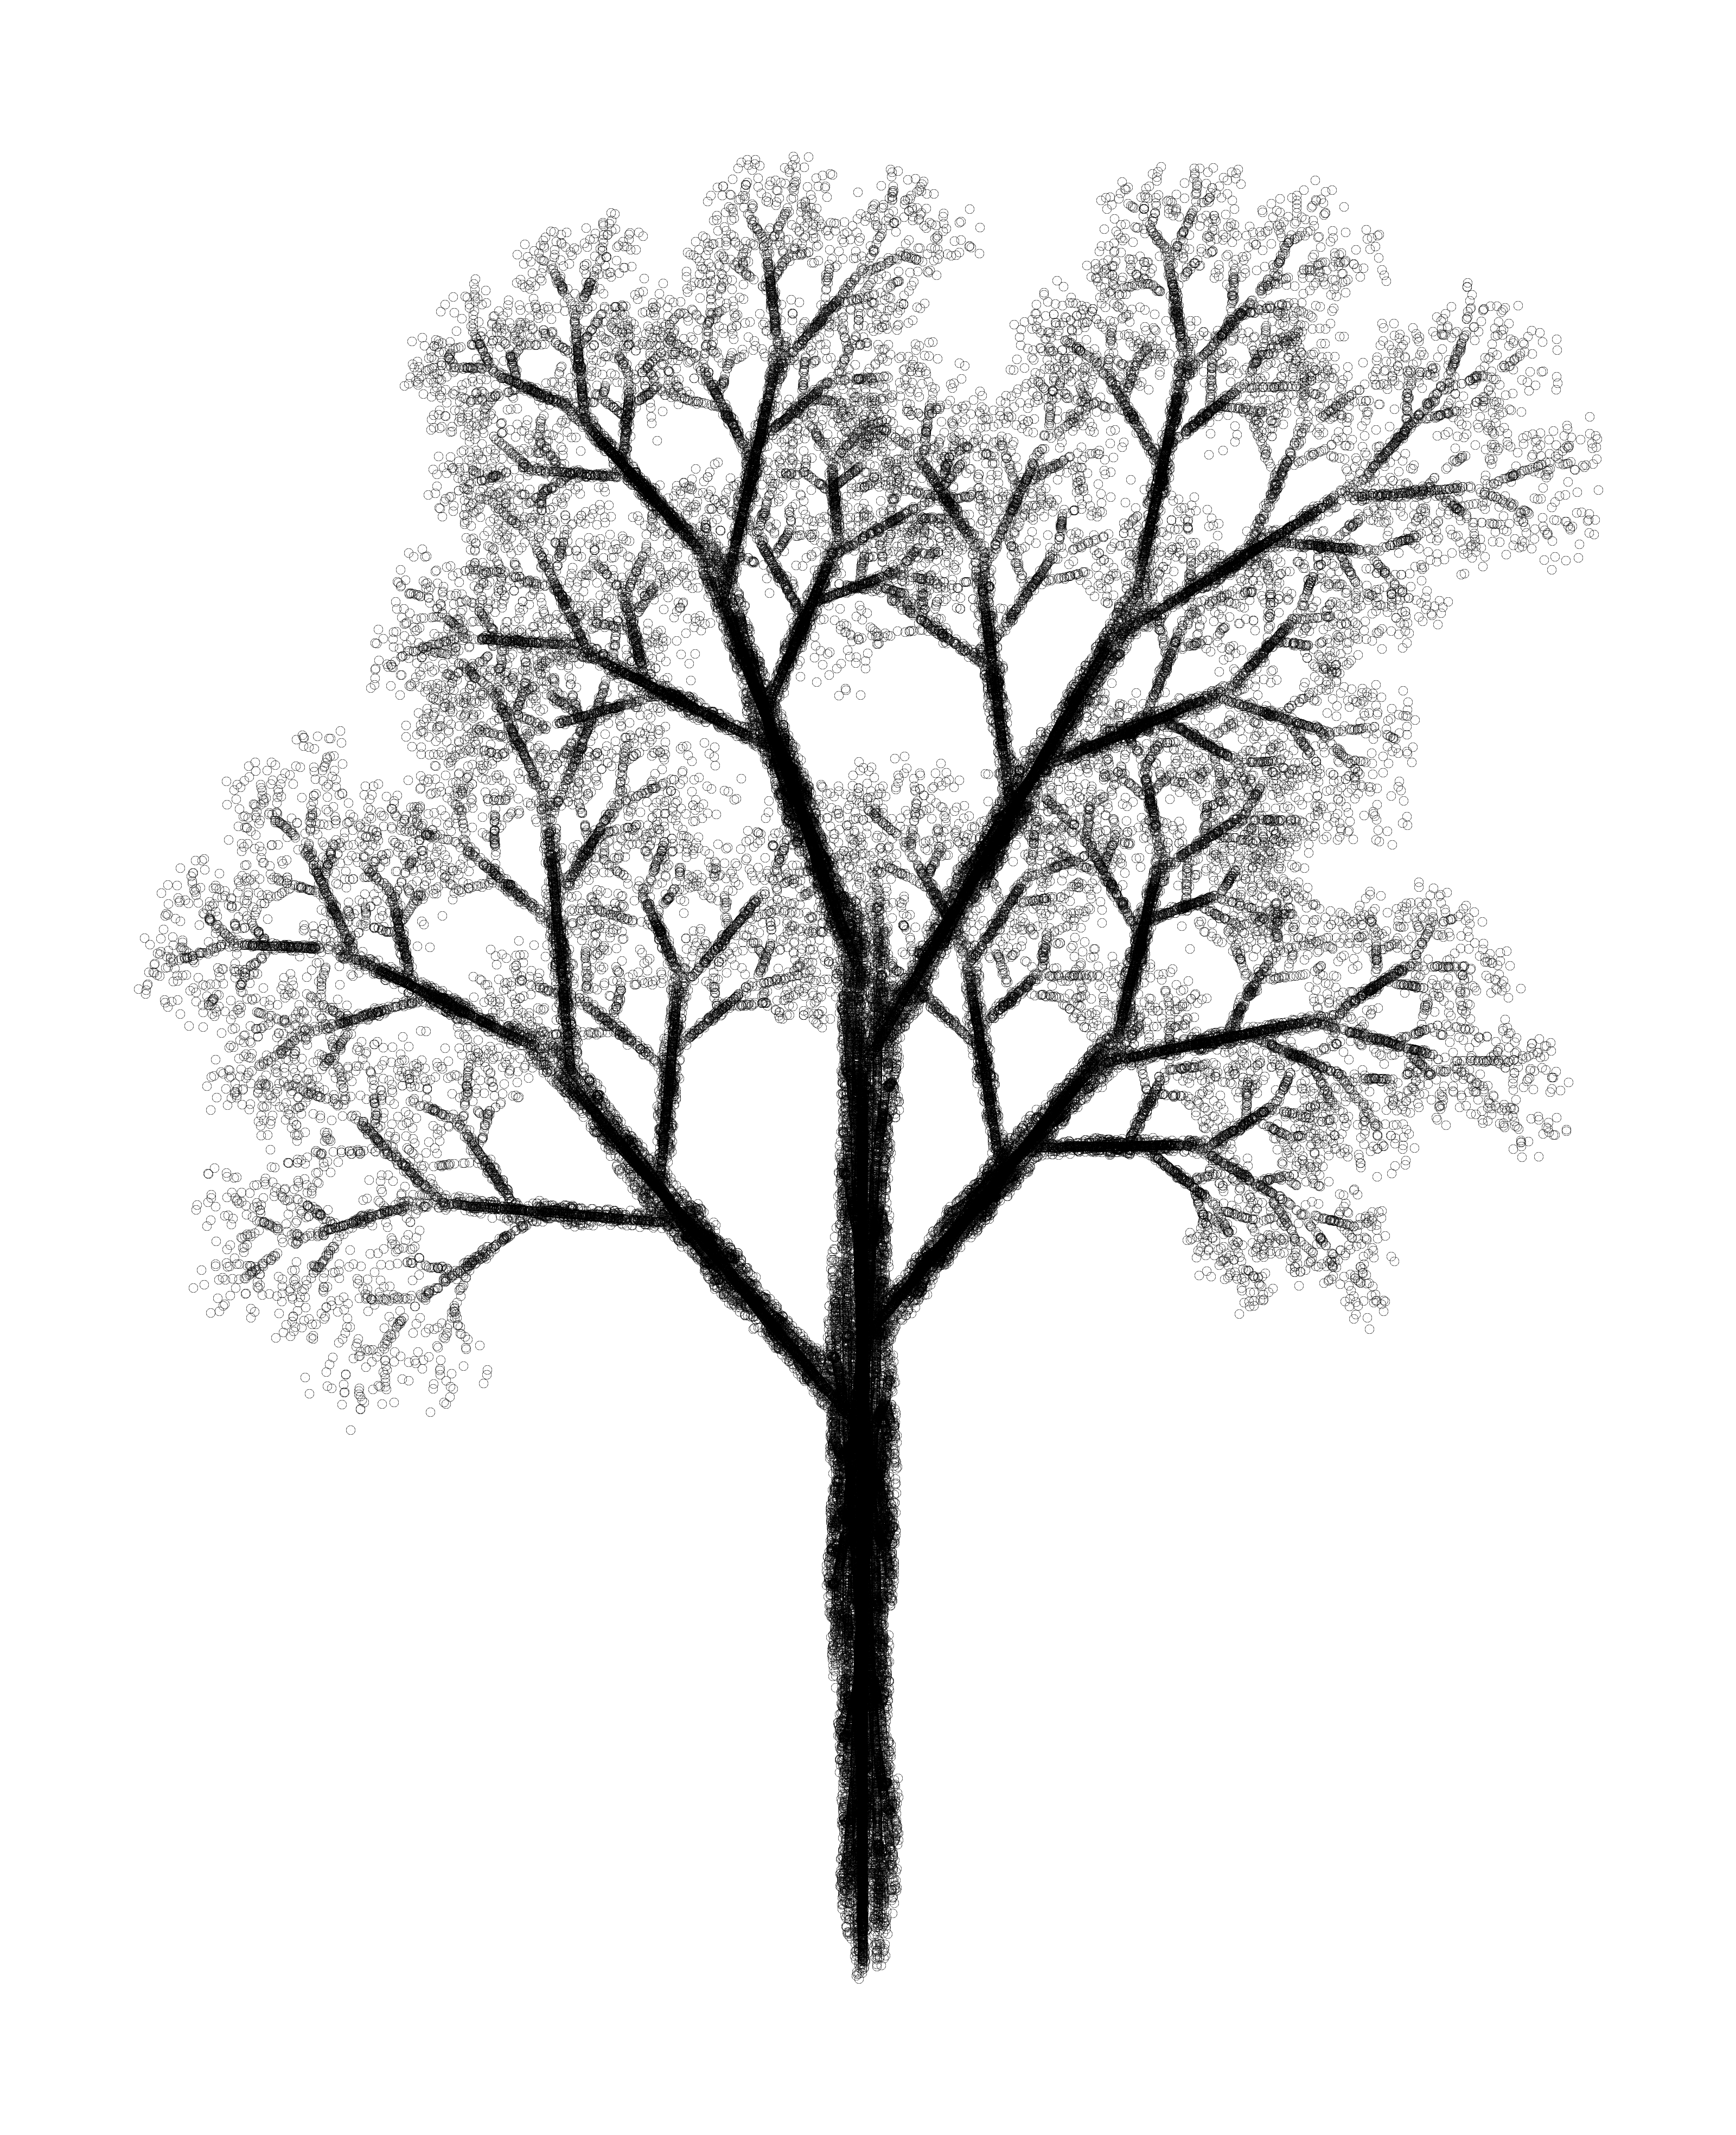
\includegraphics[width=.28\textwidth]{fractal_tree_3}
    \vfill
  \end{frame}
}

{
  \setbeamercolor{background canvas}{bg=white}
  \setbeamercolor{background canvas}{bg=white}
  \setbeamercolor{normal text}{fg=black}

  \usebeamercolor[fg]{normal text}

  \setbeamercolor{frametitle}{fg=black}
  \setbeamercolor{framesubtitle}{fg=black}
  \setbeamercolor{itemize item}{fg=black}

  \begin{frame}[fragile]{}{}
    \vfill
    \flushright
    \Large
    \textbf{\color{black} Thank you for your attention}

    \large
    \textbf{\color{gray} Any question ?}
    \vfill
  \end{frame}
}

\end{document}
